%!TEX root = ../thesis.tex
%*******************************************************************************
%*********************************** First Chapter *****************************
%*******************************************************************************

\chapter{The Theory of Neutrino Physics}\label{chap:theory}
\setlength{\epigraphwidth}{.45\textwidth}
\epigraph{\textit{Light\\Light\\The visible reminder of Invisible Light}}{\textit{The Rock}\\\textsc{T. S. Eliot}}
\setlength{\epigraphwidth}{.4\textwidth}

\section{The Standard Model and Neutrinos}
% \subsection{A Brief Introduction to the Standard Model}
% Covering how the SM works at the highest level, including:
% \begin{itemize}
%     \item Quantum Field Theory and the Lagrangian dynamical framework
%     \item The connection between symmetries of a QFT model and its gauge fields that describe the model's forces
%     \item The SM's fundamental symmetries, and associated forces, but ---
%     \item Not (exactly) what we see ``normally''! The electromagnetic and weak forces appear distinct, and the weak gauge bosons have mass. To explain this, we need a further component, the Brout-Englert-Higgs (BEH) Mechanism. 
% \end{itemize}
% [2 pages total]
% \subsection{Neutrinos within the Standard Model}
\nomenclature{\textbf{SM}}{The Standard Model of Particle Physics}
The \textit{Standard Model} (SM) of Particle Physics is the culmination of a century's work by scientists to understand the fundamental constituent elements of the Universe, and their interactions. Within the SM, fundamental particles are excitations of associated quantum fields within spacetime. One class of particles in the SM are known as the neutrinos, $\nu$: these are spin-$1/2$ fermions which are neutral in both the strong and electromagnetic force. The only means by which they are known to interact is through the weak nuclear force. There are three `flavours' of neutrino, one associated with each of their charged lepton counterparts: the electron neutrino $\nu_e$, the muon neutrino $\nu_\mu$, and the tau neutrino $\nu_\tau$.

\nomenclature{\textbf{EW}}{Electroweak (Theory)}
Crucial to understanding the nature of neutrinos is their interactions with other particles. Within the SM, the weak nuclear force and electromagnetism are unified into the Electroweak (EW) Theory by the work of Glashow, Salam, and Weinberg~\cite{glashowPartialsymmetriesWeakInteractions1961,weinbergModelLeptons1967,salamWeakElectromagneticInteractions1994}. % Cite foundational EW papers
This is a so-called \textit{chiral gauge field theory}. Gauge field theories are a special type of quantum field theory which demand that the Lagrangian density $\mathcal{L}$ is invariant under certain kinds of transformation, in addition to the usual requirement of Lorentz invariance. For EW, the Lagrangian is invariant under `local' transformations of the fields' internal degrees of freedom, defined by the `gauge' group $SU(2)_{L}\times U(1)_{Y}$, where $L$ and $Y$ are known as the left-handed weak isospin and weak hypercharge, respectively.

A local transformation is one which changes values of the fields in a manner that is dependent on the spacetime coordinates. By demanding invariance under these gauge transformations, as well as Lorentz invariance, the theory naturally predicts the existence of vector (spin-1) boson particles. These are known as the `gauge' bosons of the theory, and they mediate the interactions defined by the gauge group. The massive $W^{\pm}$ and $Z^{0}$ bosons, discovered by the UA1 and UA2 experiments in 1983~\cite{arnisonExperimentalObservationIsolated1983,bannerObservationSingleIsolated1983,arnisonExperimentalObservationLepton1983}, % CITE!!!
mediate the weak nuclear force, whilst the massless photon $\gamma$ mediates the electromagnetic force.

The theory of EW interactions is also \textit{chiral}. Any spinor that defines the wavefunction of a spin-$1/2$ field can be split into its left- and right-handed `chiral' components, defined through the projection operators $P_{L,R} = \frac{1\mp\gamma^{5}}{2}$. The force associated with the $SU(2)_{L}$ part of the EW gauge group only interacts with the left-handed components of particles, denoted with the subscript $L$ on their wavefunction.

\nomenclature{\textbf{NC}}{Neutral Current (weak interaction)}
\nomenclature{\textbf{CC}}{Charged Current (weak interaction)}
The Lagrangian that defines the weak interactions of neutrinos is:
\begin{equation}
    -\mathcal{L} = \frac{g}{2\cos{\theta_{W}}}\sum_{\ell,L}\bar{\nu}_{\ell,L}\gamma^{\mu}\nu_{\ell,L}Z^{0}_{\mu}
    +\frac{g}{\sqrt{2}}\sum_{\ell}\bar{\nu}_{\ell,L}\gamma^{\mu}\ell^{-}_{L}W^{+}_{\mu} + \mathrm{h.c.}.
\end{equation}
Here, $g$ is the dimensionless coupling constant associated with $SU(2)_{L}$, and $\theta_{W}$ is the Weinberg angle. The three lepton flavour fields are denoted by $\ell=e,\mu,\tau$, with their associated neutrino fields being given by $\nu_{\ell}$. Similarly, the fields associated with the weak gauge bosons are given by $W^{\pm}$ and $Z^{0}$. The two components of this Lagrangian are known as the Neutral Current (NC) and Charged Current (CC) weak interactions of neutrinos, respectively. Similar Lagrangians exist that define the NC and CC interactions of quarks, as well as the NC interactions of the charged leptons.

\nomenclature{\textbf{IBD}}{Inverse $\beta$-decay}
Solidifying this theoretical picture are decades-worth of experimental tests of neutrinos and their place in the SM. The first neutrinos to be detected were electron anti-neutrinos, by Cowan and Reines in 1956~\cite{cowanDetectionFreeNeutrino1956,reinesNeutrino1956}. % cite Reines and Cowen.
These neutrinos were generated in the $\beta$-decay of radioactive isotopes within the Savannah River nuclear reactor: \ce{n \to p + e^{-} + \bar{\nu}_{e}}. This decay arises from a down quark within the neutron of an atom converting into an up quark via a CC interaction, generating a virtual $W^{-}$ boson that promptly decays into an electron and $\bar{\nu}_{e}$. The method by which Cowen and Reines detected these anti-neutrinos was through \textit{inverse $\beta$-decay} (IBD): \ce{\bar{\nu}_{e} + p \to e^{+} + n}. This process also originates from CC interactions. Analogous CC interactions allowed Danby \textit{et al} to discover the muon neutrino in 1962~\cite{danbyObservationHighEnergyNeutrino1962}, % cite Lederman, Schwarts, Steinberger
and the DONUT Collaboration to discover the tau neutrino in 2000~\cite{kodamaObservationTauNeutrino2001}. % cite DONUT Collaboration

The existence of NC interactions with neutrinos and anti-neutrinos was first demonstrated by the Gargamelle experiment in 1974~\cite{hasertObservationNeutrinolikeInteractions1973,hasertSearchElasticMuonneutrino1973,hasertObservationNeutrinolikeInteractions1974,blietschauEvidenceLeptonicNeutral1976}. % cite gargamelle
In particular, the observation of anti-muon neutrino electron elastic scattering, \ce{\bar{\nu}_{\mu} + e^{-} \to \bar{\nu}_{\mu} + e^{-}} by the experiment was an unambiguous demonstration of NC interactions.

In 1958, Goldhaber \textit{et al}~\cite{goldhaberHelicityNeutrinos1958} were able to demonstrate experimentally that the helicity of electron neutrinos, i.e. the component of their spin along the direction of motion, is $-1$. No evidence of neutrinos with positive helicities (or equally, anti-neutrinos with negative helicities) exists. This stands in firm contrast to all other SM particles.

No flavours of neutrino beyond the electron, muon, or tau types have been discovered. A combined analysis of data from the four LEP experiments looking at the decay width of the $Z$ boson was able to indirectly measure the number of neutrino species that could undergo NC interactions and had masses less than one half of the $Z$ boson: $N_{\nu} = 2.9963\pm0.0074$~\cite{PrecisionElectroweakMeasurements2006,janotImprovedBhabhaCross2020}. % cite LEP papers, including update with correction!
This measurement is very strong evidence that no other `light' weakly-interacting neutrinos exist.


% \begin{itemize}
%     \item Basic description of where neutrinos fit into SM: 3 kinds of neutral fermion, the counterparts to the charged fermions. Interacts with the weak force only.
%     \item Summary of the experimental evidence for this picture: mainly, the discovery of electron anti-neutrinos by Cowan and Reines, the muon neutrino by Lederman, Schwartz, and Steinberger, and the tau neutrino by the DONUT Collaboration. Further critical experiments include the first measurement of a neutrino's helicity by Goldhaber et al. as well as Danby et al.'s demonstration that $\nu_{\mu}$ are distinct from $\nu_{e}$.
%     \item More detailed description, via Feynman diagrams, of the two fundamental modes of interaction by neutrinos with the weak force: charged- and neutral-current interactions. A brief mention of the quantitative theory that underlies description: Gashow, Salam, and Weinberg's Electroweak Theory. This explains not only the V--A structure of charged-current interactions, but also predicted accurately the nature of neutral-current interactions. (Given space constraints, I see no reason to go into much of the details of the theory, or the many experimental tests of its structure.)
% \end{itemize}

% [4 pages]
\section{Neutrino Oscillations and Neutrino Masses}
So far in this description, no attempt has been made to explain the origin of the masses of the fundamental particles. It is certainly straightforward to na\"{i}vely add a mass term such as $m_{e}\bar{e}_{L}e_{R}$ into the SM Lagrangian, where $m_e$ is the mass of the electron. However, one can show that any mass terms added will necessarily violate the $SU(2)_{L}\times U(1)_{Y}$ symmetry that defines the EW interactions~\cite{deppischChapterNeutrinosStandard2019}. % should cite something appropriate.
The weak vector bosons $W^{\pm}$ and $Z$ would then need to be massless, in contradiction with observations.

\nomenclature{\textbf{BEH}}{Brout-Englert-Higgs (Mechanism)}
The solution to this problem comes in the form of the \textit{Brout-Englert-Higgs (BEH) Mechanism}~\cite{englertBrokenSymmetryMass1964,higgsBrokenSymmetriesMasses1964,guralnikGlobalConservationLaws1964}. % cite BEH theory papers
In this Mechanism, an additional two-component ``Higgs'' field $H$ is proposed, which is able to interact with the other fields of the theory in a manner that preserves the SM gauge symmetries. One part of the added Higgs field interactions are the so-called Yukawa terms, which for interactions with leptons are given by:
\begin{equation}\label{eq:SM_yukawa_leptons}
    -\mathcal{L}_{\mathrm{Yukawa,lep}} = \sum_{\ell}y_{\ell}\bar{L}^{\ell}H\ell^{c} + \mathrm{h.c.},
\end{equation}
where $y_{\ell}$ are the ``Yukawa'' coupling constants for the three lepton flavours, $L^{\ell} = \begin{pmatrix}
    \nu_{\ell,L} \\ \ell_{L}
\end{pmatrix}$ are the left-handed lepton doublets of the SM, and $\ell^{c}$ are the right-handed charged leptons.

\nomenclature{\textbf{SSB}}{Spontaneous Symmetry Breaking}
The key to the BEH Mechanism is \textit{Spontaneous Symmetry Breaking} (SSB): the Higgs field is defined in such a way that the ground state takes a non-zero `vacuum expectation value', $v$. By doing so, the underlying gauge symmetry of the EW interactions is spontaneously broken as $SU(2)_{L}\times~U(1)_{Y}\to~U(1)_{Q}$, where $U(1)_{Q}$ is the residual electromagnetic charge conservation. The above Yukawa Lagrangian term after symmetry breaking generates the mass terms for the charged leptons:
\begin{equation}
    -\mathcal{L}_{\mathrm{Yukawa,lep}} \to \sum_{\ell}m_{\ell}\bar{\ell}_{L}\ell^{c} + \mathrm{h.c.},
\end{equation}
where $m_{\ell} = \frac{v}{\sqrt{2}}y_{\ell}$ are the charged lepton masses. Other terms associated with Higgs interactions in the SM generate mass terms for the quarks and weak vector bosons, as seen in data. A further prediction of this BEH Mechanism is the existence of a massive scalar boson known as the Higgs particle; this was discovered in 2012 by the ATLAS and CMS Collaborations~\cite{aadObservationNewParticle2012,chatrchyanObservationNewBoson2012}. %cite Higgs discovery papers

The one type of fundamental particle not covered by the above argument are neutrinos. If neutrinos were massless, then there is no issue: we observe neutrinos to have only negative helicities, which is equal to left-handed chiralities if they are massless. As the SM contains no right-handed neutrinos, no Yukawa interaction can be built to generate masses for the neutrinos. One can also demonstrate that, in the SM, neutrinos cannot even obtain masses through loop corrections~\cite{workmanReviewParticlePhysics2022}. % cite PDG review 14

This assumption of massless neutrinos appears initially consistent with the current observations of direct neutrino mass measurements. The strongest direct limits come from the KATRIN experiment, which looks at the endpoint of the tritium $\beta$-decay spectrum. The `effective'\footnote{
    KATRIN measures the `effective' mass and not the actual mass, because of the phenomenon of neutrino oscillations as described in the following sections.
} electron anti-neutrino mass was measured to be $m_{\nu} < \SI{0.8}{\eV}$ at a 90\% confidence level~\cite{akerDirectNeutrinomassMeasurement2022}. % cite https://inspirehep.net/literature/1863711
Even stronger limits are available from cosmology, by looking in part at the power spectrum of the Cosmic Microwave Background. Assuming the so-called Standard `$\Lambda$CDM' Model of Cosmology, limits on the sum of all three neutrino flavours $\sum m_{\nu}<\mathcal{O}(\SI{0.1}{\eV})$ have been achieved~\cite{divalentinoMostConstrainingCosmological2021}. % cite a couple of papers, maybe.

\subsection{The Evidence for Neutrino Oscillations}\label{sec:nu_osc_evidence}
Despite the current lack of any direct measurements, we now know that at least some neutrino flavours must have mass. This is because of the phenomenon of \textit{neutrino oscillations}, which have been observed over a variety of experiments and contexts. The critical pieces of evidence for this process are described here; the underlying mathematical model that is used to explain them quantitatively is described in Section~\ref{sec:nu_osc_phenom}.

% \subsubsection{The Solar Neutrino Problem}
\subsubsection{Solar Neutrinos}
\nomenclature{\textbf{SSM}}{Standard Solar Model}
Neutrinos are generated from the Sun as a by-product of the fusion reactions at its core. At the highest level, protons fuse into alpha particles by the overall reaction \ce{4p \to ^{4}He{} + 2e^{+} + 2\nu_{e}}, generating also $\sim\SI{25}{\MeV}$ of energy that enables the Sun to shine~\cite{bahcallNeutrinoAstrophysics1989}. % cite Bahcall Neutrino Astrophysics.
This process is known as `hydrogen burning'. The Standard Solar Model (SSM) is the current best quantitative description of stellar evolution for main sequence stars, and our Sun in particular. It covers the nuclear reactions that generate both the energy that powers the star and the changes in the relative isotopic abundances, how the energy is transported out through the star via radiation of photons and convection, and how the outward pressures caused by this radiation is balanced by gravity to maintain hydrostatic equilibrium. An introduction to the SSM can be found in~\cite{bahcallNeutrinoAstrophysics1989}. % cite Bahcall's book again.

In the Sun, two sets of nuclear reactions enable hydrogen burning to occur: the \textit{proton-proton (pp) chain} and \textit{CNO cycle}. Diagrams of these reaction chains are shown in Fig.~\ref{fig:solar_nu_chains}. In the pp chain, protons are first fused together to form a \ce{^{2}H} nucleus through the `pp' and `pep' reactions, the latter also using an electron. Both of these processes are weak interactions that generate an electron neutrino. Once a deuterium nucleus has been generated, it strongly interacts with a proton to create a \ce{^{3}He} nucleus. The dominant method for hydrogen burning to then terminate is for two \ce{^{3}He} nuclei strongly interact to generate \ce{^{4}He} and two protons.

\begin{figure}
    \centering
    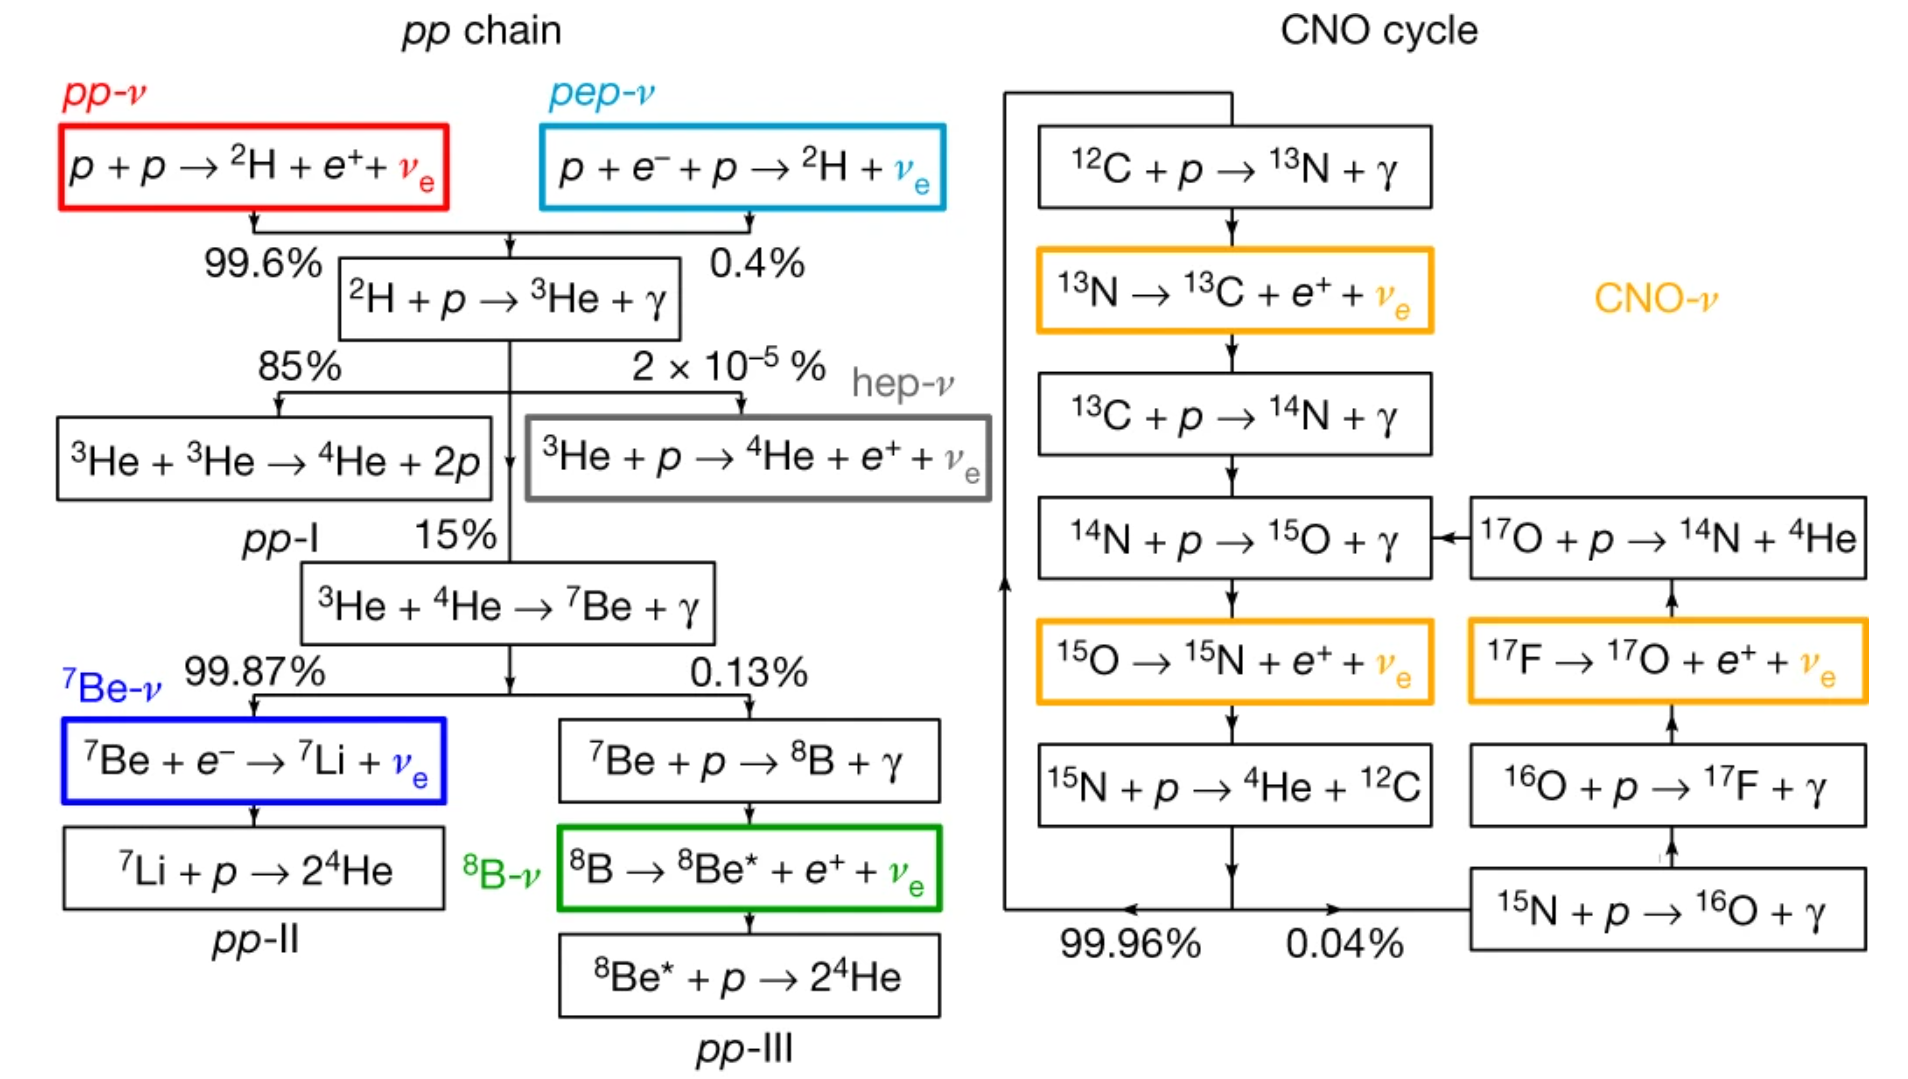
\includegraphics[width=\textwidth]{1_NeutrinoTheory/Figs/solar_nu_chains_diagram.png}
    \caption[Diagram of the pp chain and CNO cycle within the Sun]
    {Diagram of the pp chain and CNO cycle within the Sun, with the reactions that generate neutrinos highlighted. Taken from~\cite{agostiniComprehensiveMeasurementPpchain2018}.}
    \label{fig:solar_nu_chains}
\end{figure}

Two other nuclear reactions with \ce{^{3}He} are possible. In one, \ce{^{3}He} fuses with \ce{^{4}He} to generate a \ce{^{7}Be} nucleus, which can then generate a neutrino either from the creation of \ce{^{7}Li} via electron capture, or from the additional fusing into \beight{} which promptly $\beta^{+}$-decays. These are known as the \ce{^{7}Be} and \beight{} solar neutrino generation reactions, respectively. The final and rarest reaction within the pp chain that generates a neutrino is the so-called `hep' reaction, in which \ce{^{3}He} directly fuses with a proton.

The CNO cycle is a secondary means by which the Sun can burn hydrogen. This is achieved through the aid of a \ce{^{12}C} nucleus as a catalyst. Part of the cycle involves the generation of unstable isotopes \ce{^{13}N} and \ce{^{15}O}, both of which \ce{\beta^{+}}-decay, creating electron neutrinos. In a rare side-chain of the CNO cycle, it is possible to also generate \ce{^{17}F} which also weakly decays to generate a neutrino. This is the final method of generating neutrinos in our Sun.

The SSM quantitatively predicts the flux and energy spectra of neutrinos generated through each of the above processes, as incident on the Earth. This is shown in Fig.~\ref{fig:ssm_neutrino_spectra}. The shapes of the energy spectra are determined by the nuclear reactions that define the process: for example, the broad shape of the \beight{} $\nu_{e}$ energy spectrum comes from the $\beta^{+}$-decay of \beight{} isotopes, and has been measured in nuclear beam experiments to high precision~\cite{winterB8NeutrinoSpectrum2006}. % citation of B8 shape measurement by Winter et al.

\begin{figure}
    \centering
    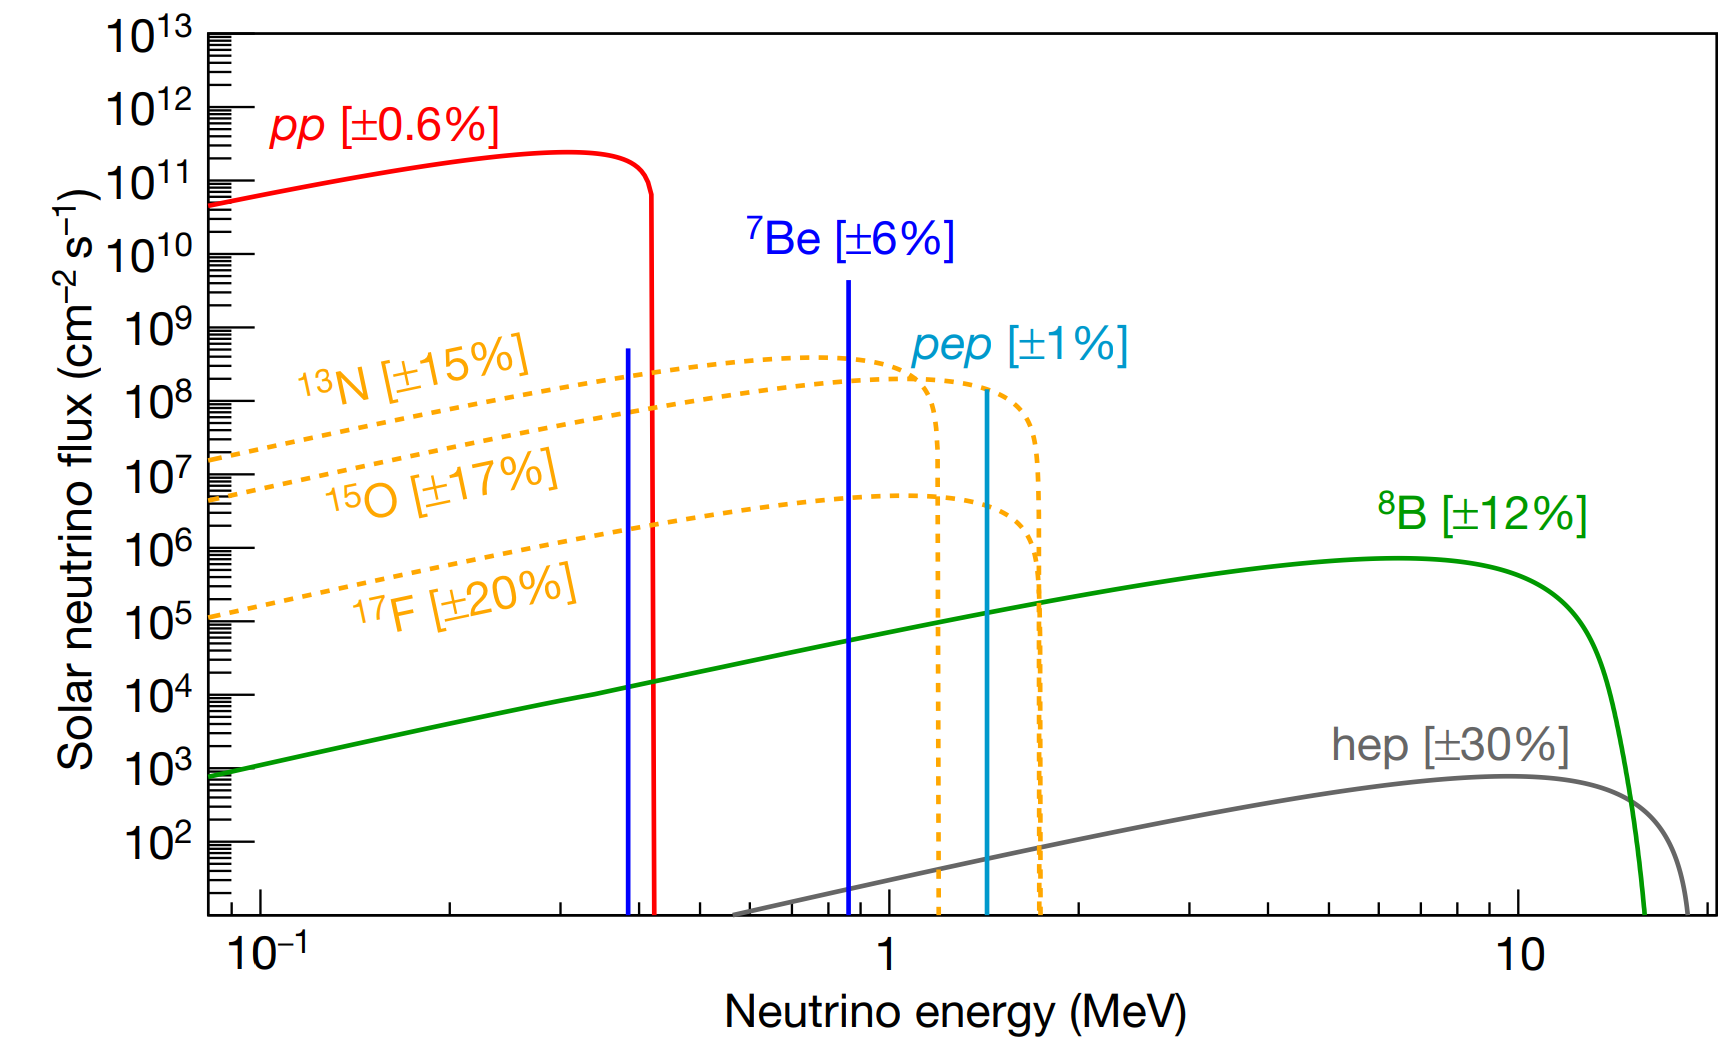
\includegraphics[width=0.8\textwidth]{1_NeutrinoTheory/Figs/solar_nu_energy_spec_SSM.png}
    \caption[Solar neutrino energy spectrum, and associated uncertainties from the SMM]
    {Solar neutrino energy spectra, and associated uncertainties from the SSM. Figure is taken from~\cite{agostiniComprehensiveMeasurementPpchain2018,vinyolesB16StandardSolar2018}; note that the flux is given in units of \si{\per\cm\squared\per\second\per\MeV} for the continuum sources, and \si{\per\cm\squared\per\second} for mono-energetic sources.}
    \label{fig:ssm_neutrino_spectra}
\end{figure}

The rate of the \beight{} decays in the Sun, and hence the generated neutrino flux, depend strongly on the radial temperature distribution of the Sun, the cross-sections of the pp chain nuclear reactions, and the Sun's chemical composition. The latter point remains a topic of some controversy: measurements of the relative abundances in 1998 through spectroscopy of the Sun's photosphere as well as meteorites give a `metal-to-hydrogen' ratio of $Z/X = 0.023$~\cite{grevesseStandardSolarComposition1998}, whereas a more recent study in 2009 has a substantially lower value of $Z/X = 0.018$~\cite{asplundChemicalCompositionSun2009}.
\footnote{`Metal' here is used in the astrophysical sense: elements heavier than hydrogen or helium.} 
These two models are called the `high-metallicity' \texttt{GS98} model and `low-metallicity' \texttt{AGSS09met} model, respectively. The current best SSM associated with these two abundance models, denoted \texttt{B16\_GS98} and \texttt{B16\_AGSS09met}, have \beight{} flux predictions of $\Phi_{\beight{}} = (5.46\pm12\%)\times 10^{6}\,\si{\per\cm\squared\per\second}$ and $\Phi_{\beight{}} = (4.50\pm12\%)\times 10^{6}\,\si{\per\cm\squared\per\second}$, respectively~\cite{vinyolesB16StandardSolar2018}.

% Rest of this subsubsection had a bunch of stuff on the history of the solar neutrino problem.
% Armin rightly points out that I can save space here by not covering this in much detail at all!
% I do need to make sure I explain neutrino-electron elastic scattering theory, though.

Since the late 1960s, a number of experiments have been able to detect solar neutrinos, using different techniques. The earliest of these was the Homestake Chlorine detector, which used the capture of electron neutrinos on \ce{^{37}Cl} nuclei to generate \ce{^{37}Ar{}} atoms that could be chemically extracted and counted~\cite{davisSearchNeutrinosSun1968}. In a similar vein, the SAGE and GALLEX/GNO experiments detected the capture of electron neutrinos on \ce{^{71}Ga}~\cite{abdurashitovMeasurementSolarNeutrino2009,altmannCompleteResultsFive2005}.


% \nomenclature{\textbf{SNU}}{Solar Neutrino Unit, defined as $10^{-36}$ neutrino interactions per second}
% The first experiment built to measure solar neutrinos was that of the Homestake Chlorine Detector, starting in the late 1960s~\cite{davisSearchNeutrinosSun1968}. A large tank of \ce{C_{2}Cl_{4}} was put deep underground, whereby electron neutrinos could be captured by the \ce{^{37}Cl} nuclei: \ce{^{37}Cl{} + \nu_{e} \to ^{37}Ar{} + e^{-}}. Through a careful chemical extraction process, any atoms of \ce{^{37}Ar} generated in the tank could be counted with an efficiency over 90\%. After running the experiment for a period of almost 30 years, a final measurement of the solar neutrino interaction rate was $2.56\pm0.16(\mathrm{stat.})\pm0.16(\mathrm{sys.})\,\mathrm{ SNU}$~\cite{clevelandMeasurementSolarElectron1998}, % cite Ray davis
% where 1 SNU (`Solar Neutrino Unit') is defined as $10^{-36}$ events per target atom per second. The results as a function of time can be seen in Fig.~\ref{fig:homestake_results}.

% \begin{figure}
%     \centering
%     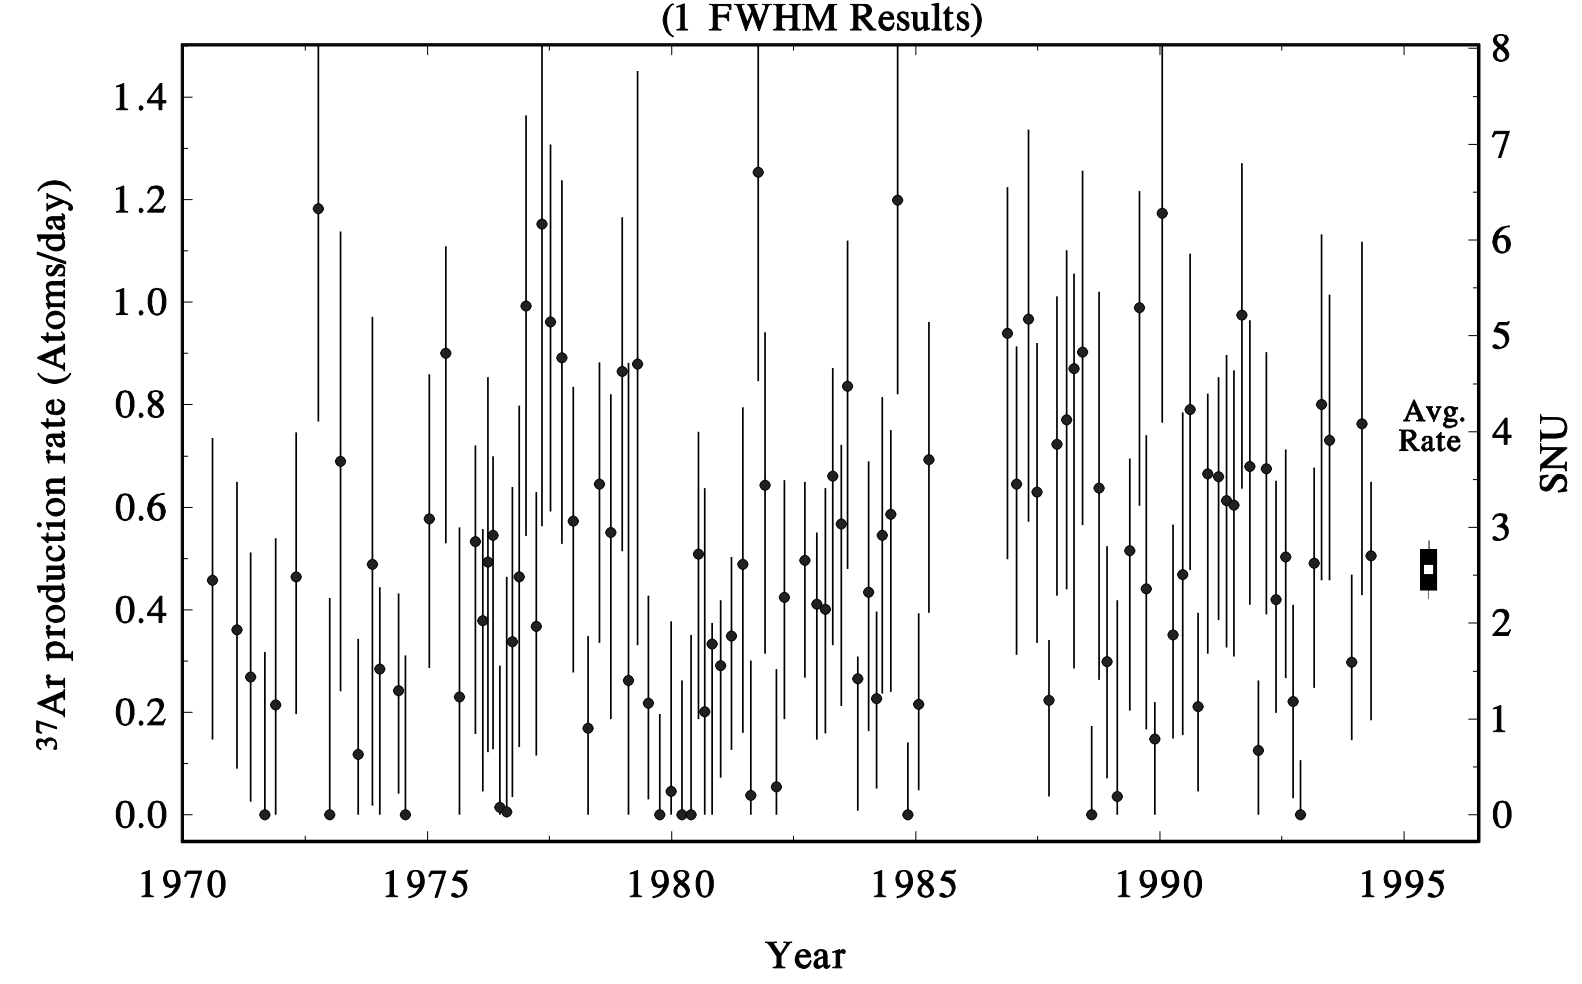
\includegraphics[width=0.8\textwidth]{1_NeutrinoTheory/Figs/homestake_summary_results.png}
%     \caption[]{Observed rate in the Homestake Chlorine detector, over the lifetime of the experiment. Taken from~\cite{clevelandMeasurementSolarElectron1998}.}
%     \label{fig:homestake_results}
% \end{figure}

% In contrast, according to one particular recent SSM using the GS98 metallicity model, the expected rate is $8.46^{+0.87}_{-0.88}\,\mathrm{ SNU}$~\cite{pena-garaySolarNeutrinosSolar2008}, highly inconsistent with the results at Homestake. This disagreement became known as the \textit{Solar Neutrino Problem}, and was the first piece of evidence towards neutrino oscillations.

% Since the Homestake experiment, a series of solar neutrino experiments used a variety of different target isotopes to measure the rate of solar neutrinos. In all cases, the measured rates were substantially below what is expected from the SSM. The SAGE and GALLEX/GNO experiments used the capture of electron neutrinos on \ce{^{71}Ga} to measure the capture rate: the final observations were $65.4^{+3.1}_{-3.0}(\mathrm{stat.})\,^{+2.6}_{-2.8}(\mathrm{sys.})\,\mathrm{ SNU}$~\cite{abdurashitovMeasurementSolarNeutrino2009} and $69.3\pm4.1\pm3.6\,\mathrm{ SNU}$~\cite{altmannCompleteResultsFive2005}, respectively. An SSM expectation is $127.9^{+8.1}_{-8.2}$~\cite{pena-garaySolarNeutrinosSolar2008}. Because the capture on \ce{^{71}Ga} has a much lower energy threshold than \ce{^{37}Cl}, these experiments were able to show that the Solar Neutrino Problem was associated with the low-energy pp neutrinos as much as the higher energy \beight{} and \ce{^{7}Be} neutrinos.

\nomenclature{\textbf{ES}}{Elastic Scattering}
The Kamiokande experiment, and its successor Super-Kamiokande, are large water Cherenkov detectors, sensitive to neutrinos through neutrino-electron elastic scattering (ES): $\nu_{x} + e^{-}\to\nu_{x} + e^{-}$. All flavours of neutrino are capable of scattering through a NC process, but there is an additional CC mode for electron neutrinos, as shown in Fig.~\ref{fig:nu_e_es_feynman_diagrams}. The differential cross-section for this interaction as a function of the scattered electron's kinetic energy $T$ is given by~\cite{bahcallSolarNeutrinosRadiative1995}: % cite Bahcall
\begin{align}\label{eq:enu_es_xsec}
    \frac{d\sigma_{\nu_{i}}}{dT} &= \frac{2G_{F}^{2}m_{e}}{\pi}\left\{
        g_{L,i}^{2}(T)\left[
            1 + \frac{\alpha}{\pi}f_{-}(z)
        \right]
        + g_{R,i}^{2}(T)(1-z)^{2}\left[
            1 + \frac{\alpha}{\pi}f_{+}(z)
        \right]\right.\nonumber\\
        &\qquad \left. {}
        -g_{R,i}(T)g_{L,i}(T)\frac{m_{e}}{E_{\nu}}\left[
            1 + \frac{\alpha}{\pi}f_{+-}(z)
        \right]
    \right\},
\end{align}
where $i = e, \mu$\footnote{
    $\frac{d\sigma_{\nu_{\mu}}}{dT} = \frac{d\sigma_{\nu_{\tau}}}{dT}$ because both flavours of neutrino only undergo the NC interaction.
}, $G_{F}$ is the Fermi coupling constant, $m_{e}$ is the electron mass, $\alpha$ is the fine-structure constant, $E_{\nu}$ is the incident neutrino energy, and $z = T/E_{\nu}$. $g_{L,R}(T)$ are the left- and right-handed running chiral couplings, which have a $T$-dependence because of radiative corrections. Similarly, $f_{-}(z)$, $f_{+}(z)$, and $f_{+-}(z)$ are all QED radiative correction terms. 
% Fig.~\ref{fig:nu_e_es_xsec} shows this differential cross-section for both $\nu_{e}$ and $\nu_{\mu}$ scattering. As can be seen, the cross-section for $\nu_{e}$ is $\sim 6$ times that of $\nu_{\mu}$, because of the additional CC interaction mode.

\begin{figure}
    \centering
    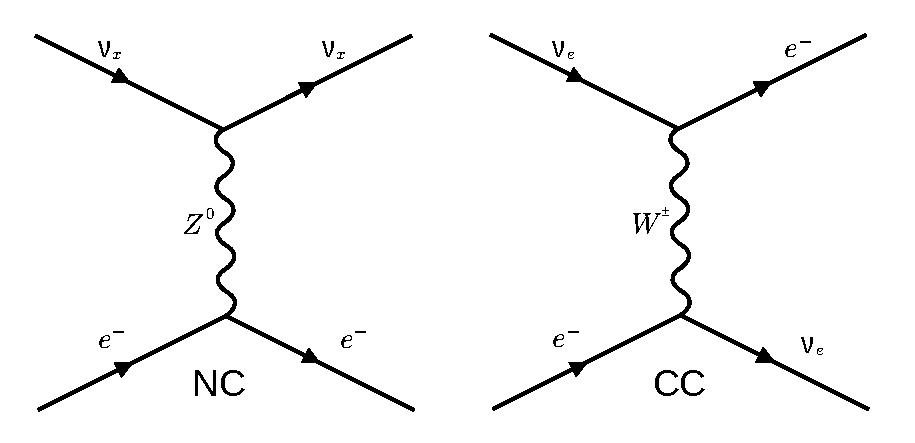
\includegraphics[width=\textwidth]{1_NeutrinoTheory/Figs/feynman_diag_nu_e_es.pdf}
    \caption[The two tree-level Feynman diagrams associated with neutrino-electron elastic scattering]
    {The tree-level Feynman diagrams associated with the NC and CC modes of neutrino-electron elastic scattering.}
    \label{fig:nu_e_es_feynman_diagrams}
\end{figure}

% \begin{figure}
%     \centering
%     % \includegraphics[]{}
%     \caption[]{}
%     \label{fig:nu_e_es_xsec}
% \end{figure}

% The most recent combined measurement of the \beight{} solar neutrino flux in Super-Kamiokande is $(2.345\pm0.014(\mathrm{stat.})\pm0.036(\mathrm{sys.}))\times10^{6}\,\si{\per\cm\squared\per\second}$~\cite{abeSolarNeutrinoMeasurements2016}, roughly half the amount expected from the SSM~\cite{vinyolesB16StandardSolar2018}.

\nomenclature{\textbf{SNO}}{Sudbury Neutrino Observatory}
\nomenclature{\textbf{UPW}}{Ultra-pure water}
A consistent finding in all of these solar neutrino experiments was that the measured rate of neutrino interactions was substantially less the expectation given by the SSM~\cite{clevelandMeasurementSolarElectron1998,abdurashitovMeasurementSolarNeutrino2009,altmannCompleteResultsFive2005,abeSolarNeutrinoMeasurements2016}. This was known as the \textit{Solar Neutrino Problem}. To solve it, the Sudbury Neutrino Observatory, SNO, was built. A large spherical acrylic vessel \SI{2.2}{\km} underground was filled with \num{1000} tonnes of heavy water, \ce{D_{2}O}, from which Cherenkov light due to particle interactions could be detected~\cite{BOGER2000172}. Neutrinos were able to interact with the heavy water via three complementary modes: the CC process \ce{\nu_{e} + d \to e^{-} + 2p}, the NC process \ce{\nu_{x} + d \to \nu_{x} + p{} + n}, and the ES process described above.

Results of the measured fluxes of $\nu_{e}$ and $\nu_{\mu,\tau}$ solar neutrinos for the three detection modes in SNO, ES results from Super-Kamiokande, and comparison to the SSM are shown in Fig.~\ref{fig:sno_flux_results}. Because the NC interaction is insensitive to neutrino flavour, it is able to directly measure the total flux of \beight{} solar neutrinos, regardless of flavour. One can see that, from the results, the NC flux measurement is consistent with the SSM. In contrast, the CC mode is only sensitive to the $\nu_{e}$ flux, whilst the ES mode is sensitive to an admixture of the different neutrino flavours. The results of all measurements of solar neutrinos from both SNO and Super-Kamiokande lead to consistent values of the flux of \beight{} neutrinos for each flavour, consistent also with the SSM.

\begin{figure}
    \centering
    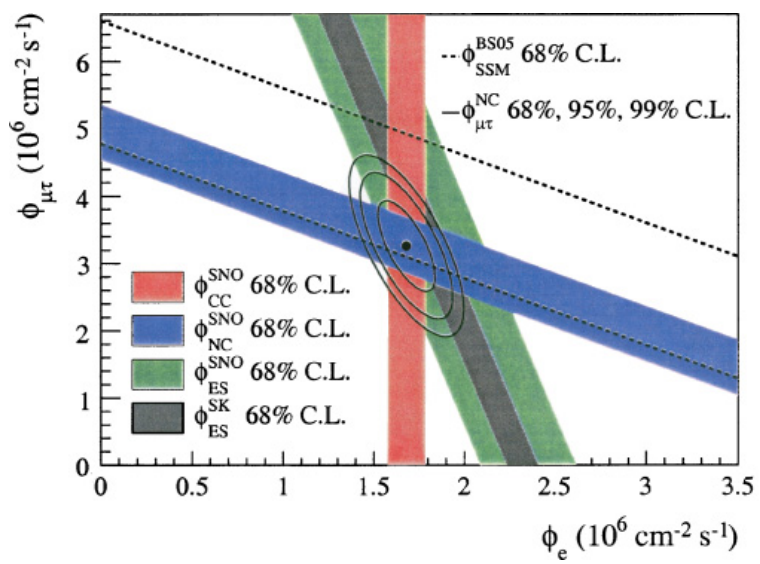
\includegraphics[width=0.7\textwidth]{1_NeutrinoTheory/Figs/sno_vs_ssm_comparison.png}
    \caption[Comparison of measured solar neutrino fluxes in the SNO CC, NC, and ES modes to the SSM]
    {Measured solar neutrino fluxes from electron neutrinos versus muon and tau neutrinos, in the SNO CC, NC, and ES modes (coloured bands). Also shown is the expectation from the SSM (dotted lines), and the ES rate measured from Super-Kamiokande (black band). The combined probability contours are shown in black. Taken from~\cite{aharmimElectronEnergySpectra2005}.}
    \label{fig:sno_flux_results}
\end{figure}

\subsubsection{Other Evidence for Neutrino Oscillations}
% Deliberately trying to be brief here! There's no real need to go into gory detail about a full play-by-play.
There are three other major areas in which neutrino oscillations have been observed. The first are atmospheric neutrinos, which come from the decays of cosmic rays in the Earth's atmosphere. In the  IBM~\cite{becker-szendyElectronMuonneutrinoContent1992}, % cite
Kamiokande~\cite{fukudaAtmosphericVmveRatio1994}, % cite
and Super-Kamiokande~\cite{fukudaEvidenceOscillationAtmospheric1998} % cite
experiments, these neutrinos were detected via CC interactions in water, with the ability to distinguish between electron and muon tracks coming from electron and muon neutrinos, respectively. It was consistently observed that the observed ratio of $\nu_{\mu}$ to $\nu_{e}$ events was consistently below expectations, a phenomenon known at the time as the \textit{Atmospheric Neutrino Anomaly}. Super-Kamiokande was able to show~\cite{ashieEvidenceOscillatorySignature2004} that the anomaly could be explained by a disappearance of muon neutrinos that depends on the ratio $L/E$, where $L$ is the estimated distance from production of the neutrino, and $E$ is the neutrino energy.

The next class of evidence comes from the detection of electron anti-neutrinos from nuclear reactors. These have consistently been detected through the use of IBD, all the way back to the first observation of neutrinos by Cowan and Reines~\cite{cowanDetectionFreeNeutrino1956,reinesNeutrino1956}. Contemporary experiments such as KamLAND~\cite{gandoReactorOnoffAntineutrino2013}, Daya Bay~\cite{adeyMeasurementElectronAntineutrino2018}, Double Chooz~\cite{dekerretDoubleChoozTh132020}, and RENO~\cite{bakMeasurementReactorAntineutrino2018}, have all measured disappearances in the rate of IBD interactions that depended in an oscillatory manner on the ratio $L/E$.

Finally, a variety of experiments have observed neutrinos that were generated from particle accelerators. In particular, the T2K~\cite{abeImprovedConstraintsNeutrino2021,abeObservationElectronNeutrino2014} and NOvA~\cite{adamsonConstraintsOscillationParameters2017,adamsonFirstMeasurementElectron2016} experiments have both been able to show the disappearance of both $\nu_{\mu}$ and $\bar{\nu}_{\mu}$ from their accelerator beams, along with the appearance of $\nu_{e}$ and $\bar{\nu}_{e}$. Recently, the two experiments have seen evidence for differences in the appearance and disappearance rates of neutrinos and antineutrinos~\cite{abeConstraintMatterAntimatter2020,aceroFirstMeasurementNeutrino2019}. In addition, the OPERA experiment was able to demonstrate the appearance of $\nu_{\tau}$ in their detector~\cite{agafonovaFinalResultsOPERA2018}.

% \subsubsection{The Atmospheric Neutrino Anomaly}
% Atmospheric neutrinos come from the decays of cosmic ray pions and muons in the Earth's atmosphere. One can show that the expected ratio of the flux of muon neutrinos to electron neutrinos generated in the atmosphere should be about 2~\cite{fukudaEvidenceOscillationAtmospheric1998}. % cite something!
% The IBM~\cite{becker-szendyElectronMuonneutrinoContent1992}, % cite
% Kamiokande~\cite{fukudaAtmosphericVmveRatio1994}, % cite
% and Super-Kamiokande~\cite{fukudaEvidenceOscillationAtmospheric1998} % cite
% experiments were able to detect atmospheric neutrinos through CC interactions with electrons in the water, generating electron or muon tracks (depending on the neutrino flavour) that could be distinguished by the shape of their Cherenkov rings. In all cases, the observed ratio of $\nu_{\mu}$ to $\nu_{e}$ events was consistently below expectations. This was known as the Atmospheric Neutrino Anomaly.

% Super-Kamiokande was able to gather enough statistics from atmospheric neutrino interactions to demonstrate that there was a clear dependence on the rate of muon neutrino interactions as a function of the event direction. In particular, the asymmetry $A$ between the number of upward-going muon neutrino events $U$, and downward-going events $D$, was measured in one dataset to be~\cite{fukudaEvidenceOscillationAtmospheric1998}: % cite SK
% \begin{equation*}
%     A = \frac{U-D}{U+D} = -0.296 \pm 0.048(\mathrm{stat.}) \pm 0.01(\mathrm{sys.}),
% \end{equation*}
% a deviation from zero by over 6$\sigma$. In contrast, the asymmetry measured for atmospheric $\nu_{e}$ events was consistent with zero. Further analysis on the experiment looked at the rate of atmospheric $\nu_{\mu}$ events as a function of the ratio $L/E$, where $L$ is the estimated distance from production of the neutrino, and $E$ is the neutrino energy. The relative rate compared to expectations is shown in Fig.~\ref{fig:LE_plot_SK_atmos}. Taken together, these atmospheric neutrino results demonstrate that there is a disappearance of muon neutrinos which depends on the ratio $L/E$, whereas there is no similar effect for the electron neutrinos.

% \begin{figure}
%     \centering
%     \begin{subfigure}{0.48\textwidth}
%         \centering
%         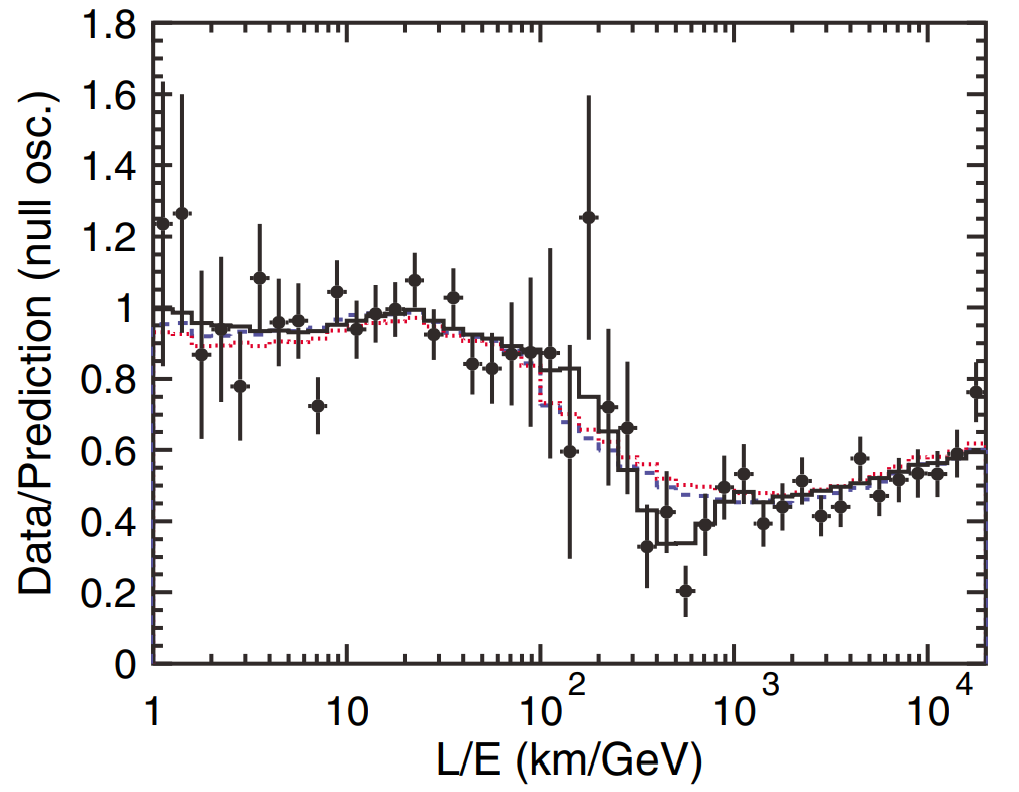
\includegraphics[width=0.95\linewidth]{1_NeutrinoTheory/Figs/sk_atmospherics_LE_plot.png}
%         \caption{}
%         \label{fig:LE_plot_SK_atmos}
%     \end{subfigure}
%     \begin{subfigure}{0.48\textwidth}
%         \centering
%         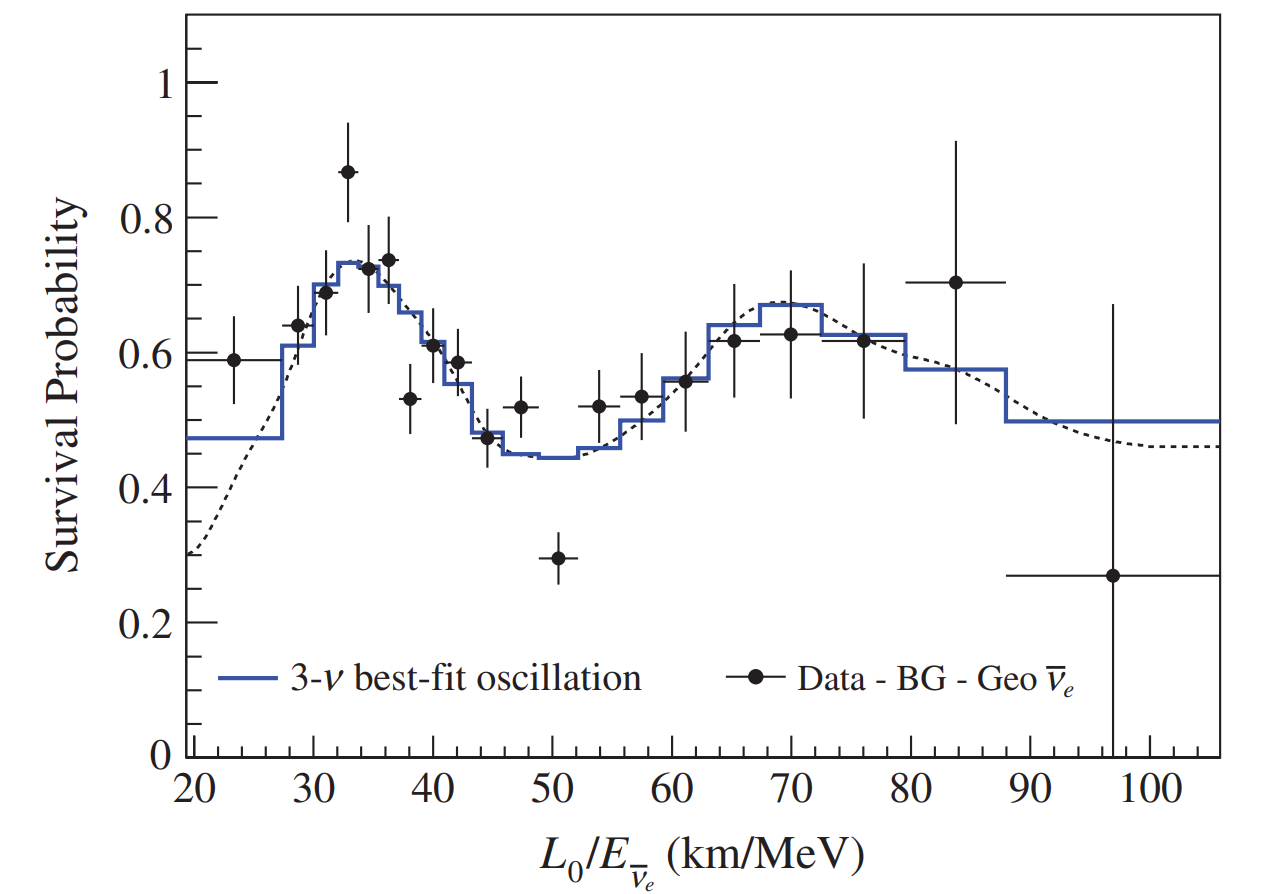
\includegraphics[width=0.95\linewidth]{1_NeutrinoTheory/Figs/kamland_reactor_LE_plot.png}
%         \caption{}
%         \label{fig:LE_plot_KamLAND_antinu}
%     \end{subfigure}
%     \begin{subfigure}{0.48\textwidth}
%         \centering
%         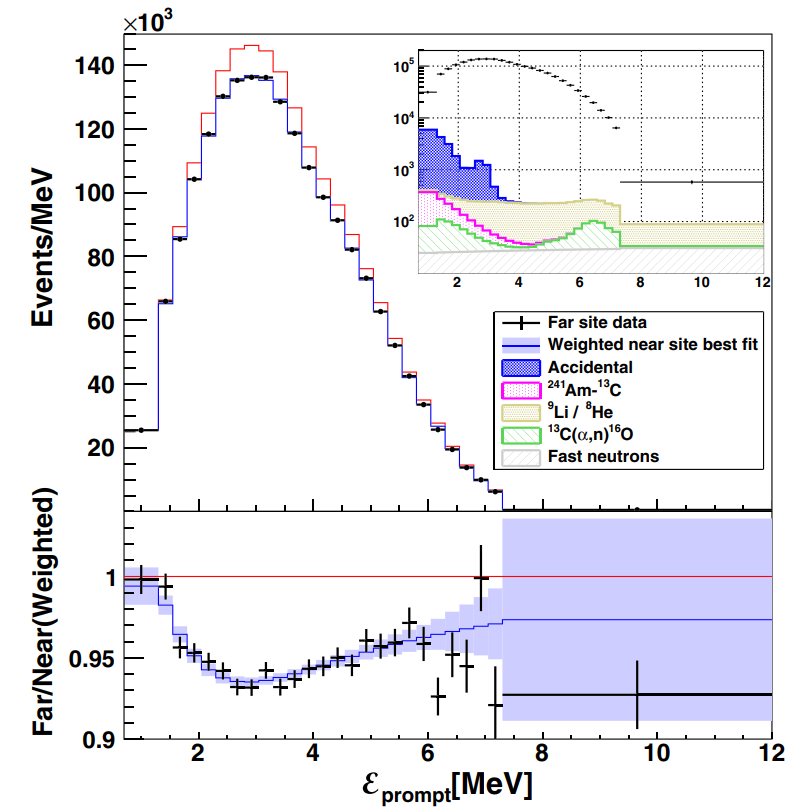
\includegraphics[width=0.95\linewidth]{1_NeutrinoTheory/Figs/dayabay_reactor_e_plot.png}
%         \caption{}
%         \label{fig:LE_plot_DayaBay}
%     \end{subfigure}
%     \begin{subfigure}{0.48\textwidth}
%         \centering
%         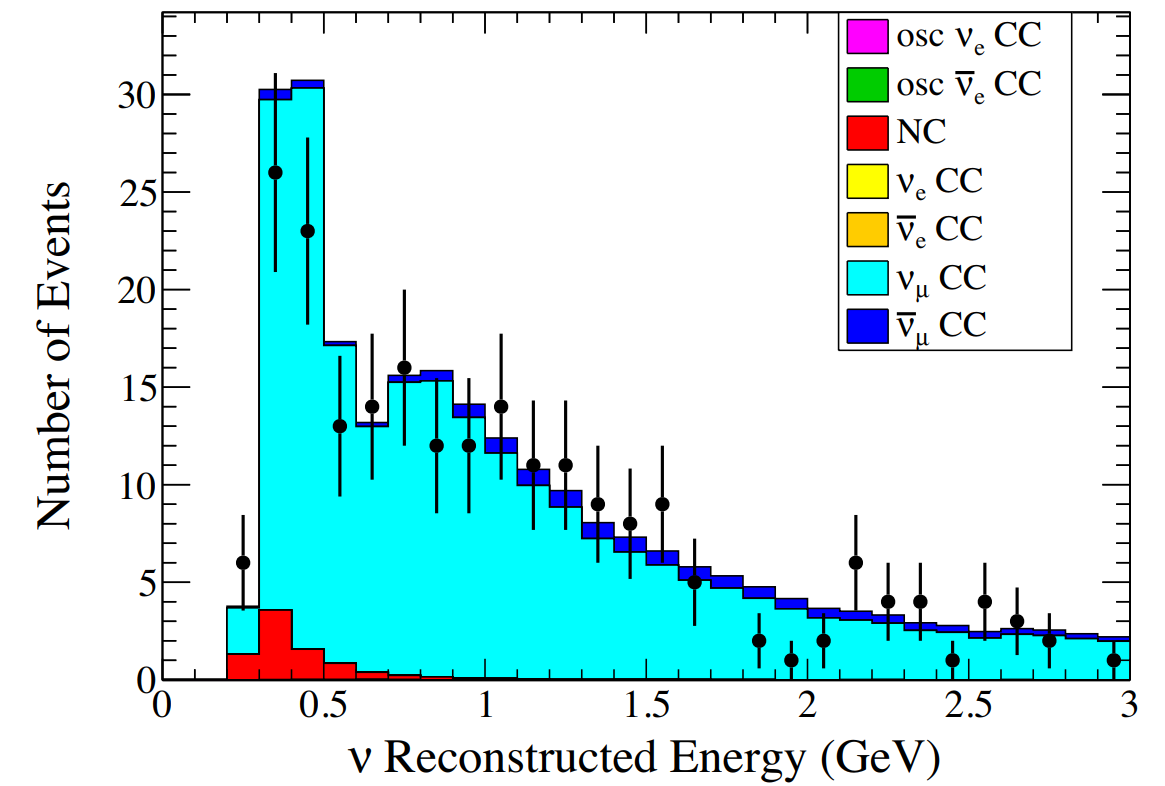
\includegraphics[width=0.95\linewidth]{1_NeutrinoTheory/Figs/T2K_numu_E_plot.png}
%         \caption{}
%         \label{fig:LE_plot_T2K_numu}
%     \end{subfigure}
%     \caption[]
%     {Plots of measured survival probability for various types of neutrinos, in different experiments, as a function of $L/E$ (or just $E$ when $L$ is fixed). \textbf{(a)}: Atmospheric neutrinos from Super-Kamiokande~\cite{ashieEvidenceOscillatorySignature2004}. The solid line indicates the best-fit expectation from 2-flavour neutrino oscillations; the dashed and dotted lines correspond to the alternative hypotheses of neutrino decay and decoherence, respectively. \textbf{(b)}: Reactor anti-neutrinos from KamLAND~\cite{gandoReactorOnoffAntineutrino2013}. $L_{0} = \SI{180}{\km}$ is the flux-weighted average reactor baseline; the blue bins and black dotted line correspond to the 3-flavour neutrino oscillation best-fit curve. \textbf{(c)}: Reactor anti-neutrinos from Daya Bay~\cite{adeyMeasurementElectronAntineutrino2018}. The expected number of events in the far site with/without neutrino oscillations (blue/red lines) based on the observations in the near site is compared to observations in the far site. \textbf{(d)}: Accelerator muon neutrinos from T2K~\cite{abeImprovedConstraintsNeutrino2021}.}
%     \label{fig:LE_plots}
% \end{figure}

% \subsubsection{Reactor Anti-neutrinos}
% The detection of $\bar{\nu}_{e}$ from nuclear reactors via IBD has been used not just to first detect the existence of neutrinos by Cowan and Reines~\cite{cowanDetectionFreeNeutrino1956,reinesNeutrino1956}, but also to provide evidence for neutrino oscillations. For example, the KamLAND experiment is a large-scale liquid scintillator detector based in Japan in which IBD events can be detected~\cite{gandoReactorOnoffAntineutrino2013}. % cite KamLAND
% The expected rate of these events could be derived from the known powers of the various Japanese nuclear reactors, as well as their distances from the experiment. The ratio of the measured rate to expectation as a function of $L_{0}/E$, where $L_{0}$ is the flux-averaged distance to the reactors, is shown in Fig.~\ref{fig:LE_plot_KamLAND_antinu}. The plot shows clear evidence of $\bar{\nu}_{e}$ disappearance, with an oscillatory dependence on $L_{0}/E$.

% The Daya Bay~\cite{adeyMeasurementElectronAntineutrino2018}, Double Chooz~\cite{dekerretDoubleChoozTh132020}, and RENO~\cite{bakMeasurementReactorAntineutrino2018} experiments are all also liquid scintillator detectors that measured IBD interactions from reactors, but unlike KamLAND they were each placed only $\sim\SI{1}{\km}$ from a nuclear reactor. Each detector observed $\bar{\nu}_{e}$ disappearance over this much shorter length scale, also with a dependence on energy. The results from Daya Bay, as an example, are shown in Fig.~\ref{fig:LE_plot_DayaBay}. Interestingly, the magnitude of the disappearance observed in these `short-baseline' reactor antineutrino experiments is different to those seen in the `long-baseline' KamLAND experiment.

% \subsubsection{Accelerator Neutrinos}
% Neutrinos generated from accelerators have been able to demonstrate numerous pieces of direct evidence for neutrino oscillations. These accelerators are able to generate very high intensity beams of $\nu_{\mu}$ and $\bar{\nu}_{\mu}$, with some background of $\nu_{e}$ and $\bar{\nu}_{e}$. Much like experiments designed for reactor antineutrino measurements, accelerator neutrino detectors tend to come in two main varieties: long- and short-baseline. Typically, long-baseline experiments have two detectors, one near to the point of neutrino generation, and the much-larger far detector where the main oscillation measurements take place. The near-detector is used to ascertain the precise composition of neutrino beam, in order to minimise systematics in the composition of the beam as well as interaction cross-sections.

% A wide variety of accelerator neutrino experiments have taken place over the past 25 years. The long-baseline experiments T2K and NOvA have both demonstrated disappearance of both $\nu_{\mu}$ and $\bar{\nu}_{\mu}$ from their accelerator beams with high statistical significance~\cite{abeImprovedConstraintsNeutrino2021,adamsonConstraintsOscillationParameters2017}. % cite T2K, Nova
% An example of the observed energy spectrum from a predominantly $\nu_{\mu}$-type beam, as seen by T2K, is shown in Fig.~\ref{fig:LE_plot_T2K_numu}. In contrast to the energy spectrum of the neutrinos at production, which is unimodal, this plot shows oscillations in the observed rate as a function of neutrino energy. 

% T2K and NOvA have also been able to observe the appearance of $\nu_{e}$ and $\bar{\nu}_{e}$ (as appropriate) in their far detectors, well above the background rate expected~\cite{abeObservationElectronNeutrino2014,adamsonFirstMeasurementElectron2016}. Recently, the two experiments have seen evidence for differences in the appearance and disappearance rates of neutrinos and antineutrinos~\cite{abeConstraintMatterAntimatter2020,aceroFirstMeasurementNeutrino2019}. % cite CP violation papers.
% In addition to the appearance of $\nu_{e}$ shown by T2K and NOvA, the OPERA long-baseline neutrino experiment was able to show the appearance of $\nu_{\tau}$ in detector~\cite{agafonovaFinalResultsOPERA2018}. % cite OPERA
 
% short-baseline neutrino anomaly???

% \begin{itemize}
%     \item Describe status quo ante of massless nature of neutrinos: BEH mechanism as exists cannot allow for neutrinos to have mass as only left-handed neutrinos have been observed.
%     \item Furthermore, strong experimental limits on neutrino masses, from e.g. tritium-decay endpoint measurements by the KATRIN experiment and cosmological inferences from the CMB by the Planck satellite.
%     \item But --- then neutrino oscillations are observed over a variety of experiments and contexts. Summarise critical bits of evidence:
%     \item Electron neutrino disappearance in solar neutrino experiments, including Ray Davis' Homestake experiment, the SAGE/GALLEX experiments, and SNO. For the latter, the comparison of charged-current and neutral-current modes of interaction was clear evidence of neutrino oscillations over other types of process (e.g. neutrino decay).
%     \item Include in the above a brief description of Bahcall's Standard Solar Model.
%     \item Muon neutrino disappearance in atmospheric and long-baseline accelerator neutrino experiments, such as Super-Kamiokande, T2K, and No$\nu$a.
%     \item A few further observations to note are: reactor electron anti-neutrino disappearance from both KamLAND and Daya Bay; tau neutrino appearance at the OPERA experiment; short-baseline neutrino anomaly within LSND and MiniBooNE (with recent contrary evidence from MicroBooNE).
% \end{itemize}
% [5 pages]
\subsection{The Phenomenology of Neutrino Oscillations}\label{sec:nu_osc_phenom}
\subsubsection{Oscillations in Vacuum}\label{sec:nu_osc_phenom_vacuum}
Taken together, the observations described in the previous section naturally lead to the notion of neutrino oscillations: the idea that as neutrinos propagate through space they are capable of changing flavour. Special Relativity precludes massless particles from experiencing time evolution, so any theory of neutrinos changing flavour between one another must require non-zero mass states.

\nomenclature{\textbf{PMNS}}{Pontecorvo-Maki-Nakagawa-Sakata (neutrino mixing matrix)}
The initial theories describing neutrino oscillations were made by Pontecorvo, Maki, Nakagawa, and Sakata in the 1960s~\cite{makiRemarksUnifiedModel1962,pontecorvoNeutrinoExperimentsProblem1968}. % cite PMNS papers
These theories initially assumed a two-neutrino model of oscillations, but now that $\nu_{\tau}$ particles have been observed a three-neutrino model has been adopted. The theory starts by assuming that the flavour eigenstates of neutrinos, $\nu_{e,\mu,\tau}$ are different from the neutrino mass eigenstates, $\nu_{1,2,3}$, and are instead related to one another through the Pontecorvo-Maki-Nakagawa-Sakata (PMNS) mixing matrix, $U$:
\begin{align}
    \begin{pmatrix}
        \nu_{e} \\ \nu_{\mu} \\ \mu_{\tau}
    \end{pmatrix}
     &= U \cdot 
     \begin{pmatrix}
        \nu_{1} \\ \nu_{2} \\ \nu_{3}
    \end{pmatrix}
     = \begin{pmatrix}
        U_{e1} & U_{e2} & U_{e3} \\
        U_{\mu1} & U_{\mu2} & U_{\mu3} \\
        U_{\tau1} & U_{\tau2} & U_{\tau3} 
    \end{pmatrix} \cdot 
     \begin{pmatrix}
        \nu_{1} \\ \nu_{2} \\ \nu_{3}
    \end{pmatrix}.
    % &= \begin{pmatrix}
    %     c_{12}c_{13} & s_{12}c_{13} & s_{13}e^{-i\delta_{CP}} \\
    %     -s_{12}c_{23}-c_{12}s_{13}s_{23}e^{i\delta_{CP}} & c_{12}c_{23}-s_{12}s_{13}s_{23}e^{i\delta_{CP}} & c_{13}s_{23} \\
    %     s_{12}s_{23}-c_{12}s_{13}c_{23}e^{i\delta_{CP}} & -c_{12}s_{23}-s_{12}s_{13}c_{23}e^{i\delta_{CP}} & c_{13}c_{23} 
    % \end{pmatrix} \cdot 
    %  \begin{pmatrix}
    %     \nu_{1} \\ \nu_{2} \\ \nu_{3}
    % \end{pmatrix}.
\end{align}
Because $U$ must be unitary in order to preserve total probability, its components can be parameterised as follows:
\begin{equation}
    U = 
    \begin{pmatrix}
        c_{12}c_{13} & s_{12}c_{13} & s_{13}e^{-i\delta_{CP}} \\
        -s_{12}c_{23}-c_{12}s_{13}s_{23}e^{i\delta_{CP}} & c_{12}c_{23}-s_{12}s_{13}s_{23}e^{i\delta_{CP}} & c_{13}s_{23} \\
        s_{12}s_{23}-c_{12}s_{13}c_{23}e^{i\delta_{CP}} & -c_{12}s_{23}-s_{12}s_{13}c_{23}e^{i\delta_{CP}} & c_{13}c_{23} 
    \end{pmatrix} \cdot 
     \begin{pmatrix}
        \nu_{1} \\ \nu_{2} \\ \nu_{3}
    \end{pmatrix}.
\end{equation}
This matrix uses three ``mixing angles'' $0\leq \theta_{12},\theta_{13},\theta_{23}\leq \pi/2$, and one further parameter called the ``CP-violating phase'', $0\leq\delta_{CP}\leq2\pi$, with the abbreviations $s_{ij}=\sin{\theta_{ij}}$ and $c_{ij}=\cos{\theta_{ij}}$ used in the above expression.

Given that a neutrino flavour eigenstate $\Ket{\nu_{\alpha}(0)}$ ($\alpha=e,\mu,\tau$) is produced in some CC process at time $t = 0$, because mass eigenstates $\Ket{\nu_{i}(0)}$ ($i=1,2,3$) are simultaneously the energy eigenstates when propagating in free space, the time evolution of the neutrino state is given by:
\begin{equation}
    \Ket{\nu_{\alpha}(t)} = \sum_{i=1}^{3}U_{\alpha i}e^{-E_{i}t}\Ket{\nu_{i}(0)}.
\end{equation}
$E_{i}$ is the energy eigenvalues corresponding to the associated mass eigenstates. The oscillation probability of going from one flavour $\alpha$ to another $\beta$ is given by $P\left(\nu_{\alpha}\to\nu_{\beta}\right) = |\Braket{\nu_{\beta} | \nu_{\alpha}(t)}|^{2}$. Assuming that the neutrino is ultra-relativistic so that $E_{i}\gg m_{i}$, where $m_{i}$ is the mass of the $i^{\mathrm{th}}$ mass eigenstate, and that all mass eigenstates have the same definite momentum, one can show that the oscillation probability becomes~\cite{deppischChapterNeutrinoOscillations2019}: % cite Deppisch book?
\begin{align}\label{eq:nu_osc_vacuum}
    P\left(\nu_{\alpha}\to\nu_{\beta}\right) &=
        \delta_{\alpha\beta} 
        - 4\sum_{i<j}\operatorname{Re}\left\{W_{\alpha\beta,ij}\right\}\sin^{2}\left(\frac{\Delta m^{2}_{ij}L}{4E}\right)\nonumber\\
        &- 2\sum_{i<j}\operatorname{Im}\left\{W_{\alpha\beta,ij}\right\}\sin\left(\frac{\Delta m^{2}_{ij}L}{2E}\right),
\end{align}
where $\delta_{\alpha\beta}$ is the usual Kronecker delta, $W_{\alpha\beta,ij}=U_{\alpha i}U_{\beta i}^{*}U_{\alpha j}^{*}U_{\beta j}$, $\Delta m^{2}_{ij}=m^{2}_{i} - m^{2}_{j}$, $L$ is the distance between the creation and detection of the neutrinos, and $E_{i}\approx E$ is the average energy of the neutrino. As can be seen, the probability will oscillate as a function of $L/E$, in accordance with what was seen in Section~\ref{sec:nu_osc_evidence}.

If anti-neutrinos are produced, then oscillations are governed by $U^{*}$, which is equivalent to $U$ but with the CP phase changing sign: $\delta_{CP}\to -\delta_{CP}$. Therefore, the difference between $P\left(\nu_{\alpha}\to\nu_{\beta}\right)$ and $P\left(\bar{\nu}_{\alpha}\to\bar{\nu}_{\beta}\right)$ is given by twice the third term of Eq.~\ref{eq:nu_osc_vacuum}.

In a neutrino flavour disappearance measurement, $P_{\alpha\alpha} = P\left(\nu_{\alpha}\to\nu_{\beta}\right)$ is the \textit{survival probability} of the neutrinos. In this case, $W_{\alpha\beta,ij} = |U_{\alpha i}U_{\alpha j}^{*}|^{2}$ is real, and the survival probability formula simplifies to:
\begin{equation}
    P_{\alpha\alpha} = 1 
    - 4\sum_{i<j}|U_{\alpha i}U_{\alpha j}^{*}|^{2}\sin^{2}\left(\frac{\Delta m^{2}_{ij}L}{4E}\right).
\end{equation}

An experiment is only sensitive to neutrino oscillations from mass splitting $\Delta m^{2}_{ij}$ if $X_{ij}$ is $\mathcal{O}(1)$, where $X_{ij}$ is the phase within the relevant oscillation probability term:
\begin{equation}\label{eq:nu_osc_phase}
    X_{ij} = \frac{\Delta m^{2}_{ij} L}{4E} = 1.27 \frac{\Delta m^{2}_{ij} [10^{-3}\,\si{\eV\squared}] L [\si{\km}]}{E [\si{MeV}]}.
\end{equation}
If $X_{ij}\ll 1$, then $\sin^{2}\left(X_{ij}\right)\to 0$, and no oscillations are seen due to that mass splitting. If instead $X_{ij}\gg 1$, then as detectors have limited distance and energy resolutions, what can only be observed is the average effect over many oscillations, $\left<\sin^{2}\left(X_{ij}\right)\right> = 1/2$.

From the results of a variety of neutrino oscillation experiments, the oscillation parameters and magnitudes of the mass splittings have now been measured, with varying degrees of precision. A global fit of the experimental data by the NuFit group in October 2021~\cite{estebanFateHintsUpdated2020} give the values shown in Table~\ref{tab:nufit_osc_params}. All the parameters appear to have no-zero values, implying that mixing between all neutrino flavours is possible. Furthermore, $|\dmsq{}|\ll|\Delta m^{2}_{31}|\sim|\Delta m^{2}_{32}|$, meaning there are two distinct `scales' in $L/E$ that are sensitive to neutrino oscillations: $L/E\sim\SI{10}{\km\per\MeV}$ and $L/E\sim\SI{0.3}{\km\per\MeV}.$

\begin{table}
    \centering
    \begin{tabular}{c p{2.2cm} p{2.2cm}}
        \hline
        Parameter   & Normal Hierarchy                       & Inverted Hierarchy  \\ \hline \hline
        $\theta_{12} [^{\circ}]$ & $33.44^{+0.77}_{-0.74}$  & $33.45^{+0.77}_{-0.74}$     \\
        $\theta_{23} [^{\circ}]$ & $49.2^{+1.0}_{-1.3}$     & $49.5^{+1.0}_{-1.2}$  \\
        $\theta_{13} [^{\circ}]$ & $8.57^{+0.13}_{-0.12}$   & $8.60^{+0.12}_{-0.12}$  \\
        $\delta_{CP} [^{\circ}]$ & $194^{+52}_{-25}$        & $287^{+27}_{-32}$   \\
        $\dmsq{} [10^{-5}\,\si{eV\squared}]$ & $7.42^{+0.21}_{-0.20}$ & $7.42^{+0.21}_{-0.20}$    \\
        $\Delta m^{2}_{3\ell} [10^{-3}\,\si{eV\squared}]$ & $+2.515^{+0.028}_{-0.028}$ & $-2.498^{+0.028}_{-0.029}$    \\
        \hline
    \end{tabular}
    \caption[Global Fit neutrino oscillation parameters]
    {Global fit results for the neutrino oscillation parameters and mass splittings, as performed in NuFit 5.1~\cite{estebanFateHintsUpdated2020}. The results for both the Normal and Inverted Hierarchy are shown: $\Delta m^{2}_{3\ell} = \Delta m^{2}_{31}$ in the former, $\Delta m^{2}_{32}$ in the latter. The results used do not include atmospheric neutrino data from Super-Kamiokande.}
    \label{tab:nufit_osc_params}
\end{table}

\nomenclature{\textbf{IH}}{Inverted Hierarchy (of neutrino masses)}
\nomenclature{\textbf{NH}}{Normal Hierarchy (of neutrino masses)}
In addition to this information, we also know from solar data that the sign of \dmsq{} must be positive, due to the MSW Effect: this will be explained in the next section. However, the same cannot be yet said for $\Delta m^{2}_{31}$. This leads to two possible scenarios of the ordering of the neutrino mass states. If the sign of $\Delta m^{2}_{31}$ is positive, then $m_{\nu_{1}}<m_{\nu_{2}}<m_{\nu_{3}}$, known as the Normal Hierarchy (NH). Alternatively, $m_{\nu_{3}}<m_{\nu_{1}}<m_{\nu_{2}}$, known as the Inverted Hierarchy (IH).

\subsubsection{Neutrino Oscillations in Matter}
Considering only neutrino oscillations in vacuum is insufficient to understanding the results of certain neutrino experiments, especially those detecting high-energy solar neutrinos, such as those from the \beight{} chain. Using Eq.~\ref{eq:nu_osc_phase} for the case of solar neutrinos, one finds that $X_{ij}\gg 1$ for all $i,j$, so all effects of neutrino oscillations in the vacuum should be washed out. This leads to an expected electron neutrino survival probability for solar neutrinos of:
\begin{align}\label{eq:solar_pee_naive}
    P_{ee}  &= 1 - 2\sum_{i<j}|U_{ei}U_{ej}^{*}|^{2}\\
            &= 1 - \frac{1}{2}\sin^{2}(2\theta_{13}) - \frac{1}{2}\sin^{2}(2\theta_{12})\cos^{4}(\theta_{13})\\
            &= 0.55,
\end{align}
using the parameters in Table~\ref{tab:nufit_osc_params}. This survival probability value appears somewhat consistent with those measured in low-energy solar neutrino experiments such as SAGE and GALLEX/GNO, but not with experiments with higher energy thresholds such as Homestake, Super-Kamiokande, or SNO.

\nomenclature{\textbf{MSW effect}}{Mikheyev-Smirnov-Wolfenstein effect (of neutrinos)}
The resolution of this apparent problem is that the effect of matter on neutrino oscillations have not been considered. When neutrinos travel through a medium, the electrons, protons, and neutrons within that medium interact weakly with those neutrinos, leading to coherent forward elastic scattering. The resulting phenomenon is known as the \textit{MSW effect}, after its discovery by Mikheyev, Smirnov, and Wolfenstein~\cite{wolfensteinNeutrinoOscillationsMatter1978,mikheyevResonantAmplificationOscillations1986}. %cite MSW effect papers

One can show~\cite{giuntiChapterNeutrinoOscillations2007} that there is an effective potential due to the CC weak interactions from the electrons within the medium of the form $V_{CC}(x) = \sqrt{2}G_{F}n_{e}(x)$, where $n_{e}(x)$ is the electron number density at a position $x$. This effective potential is only felt by electron neutrinos, because of the additional CC interaction possible, as seen in Fig.~\ref{fig:nu_e_es_feynman_diagrams}. All neutrino flavours experience NC interactions identically, and so the effective potential generated by NC interactions from electrons, protons, and neutrons can be ignored in what follows. The effective potential modifies the Hamiltonian, and therefore by the Schr\"{o}dinger Equation the propagation of the neutrino wavefunctions are modified.

The resulting dynamics of the MSW effect for 3-$\nu$ oscillations in a general medium can become quite complex. However, for the case of solar neutrinos two simplifying assumptions can be made that make many of the equations far more tractable: a full discussion can be read in e.g.~\cite{giuntiChapter13Phenomenology2007}. % cite Giutti
Firstly, for solar neutrinos it can be shown that $A_{CC} = 2EV_{CC} \ll \Delta m^{2}_{31}$, leading to the evolution of the $\nu_{3}$ state decoupling from the $\nu_{1}$ and $\nu_{2}$ states. There exists a new basis in which the Hamiltonian is diagonalised, known as the matter eigenstate basis, leading to new effective oscillation parameters: %cite Giutti
\begin{align}\label{eq:matter_osc_params}
    \tan{2\theta_{12}^{M}} &= \frac{\tan{2\theta_{12}}}{1-\frac{A_{CC}}{A_{res}}},\nonumber\\
    \Delta m^{2}_{M,21} &= \dmsq{}\sqrt{\sin^{2}2\theta_{12} + \cos^{2}2\theta_{12}\left(1-\frac{A_{CC}}{A_{res}}\right)^{2}},\\
    A_{res} &= \frac{\cos{2\theta_{12}\dmsq{}}}{\cos^{2}\theta_{13}}.\nonumber
\end{align}
$A_{res}$ is the value of $A_{CC}$ at which a resonance occurs, leading to the effective mass splitting $\Delta m^{2}_{M,21}$ being minimised. In the core of the Sun, this resonance occurs at an energy of $E\sim \SI{2}{\MeV}$. If $A_{CC} \ll A_{res}$, then the effective oscillation parameters reduce back to the vacuum oscillation parameters, as expected. If instead $A_{res} \ll A_{CC} \ll \Delta m^{2}_{31}$, then $\theta_{12}^{M}\to \pi/2$. In this case, $\nu_{e}$ that are created in the medium are completely driven into the $\ket{\nu_{2}^{M}}$ effective mass eigenstate.

Because the values of the effective oscillation parameters are a function of the electron density of the medium, calculating the full impact of the MSW effect of a medium with strongly-changing density can be challenging. However, If the rate of change of electron density is slow enough as a function of distance, a second approximation can be made: this is known as the \textit{adiabatic approximation}. For solar neutrinos, this approximation has been shown to be valid assuming the SSM and the measured values of the oscillation parameters. Under this approximation, states that are in a given effective mass eigenstate smoothly transform into one another as the neutrinos propagate. Therefore, an electron neutrino with energies $\gg\SI{2}{\MeV}$ will have been driven into the $\ket{\nu_{2}^{M}}$ state in the Sun's core, and then smoothly transformed into the equivalent $\ket{\nu_{2}}$ mass eigenstate once it has reached the Sun's surface. This state then travels through space without any further oscillations occurring, because the neutrino has been transformed into a mass eigenstate. For such a neutrino, the detection probability becomes simply:
\begin{align}
    P(\nu_{2}\to\nu_{e}) &= |\Braket{\nu_{e}|\nu_{2}}|^{2} = |U_{e2}|^{2}\\
                         &= \sin^{2}\tonetwo{}\cos^{2}\theta_{13}\\
                         &= 0.30,
\end{align}
using the oscillation parameters from Table~\ref{tab:nufit_osc_params}. This survival probability is almost half of the value seen in Eq.~\ref{eq:solar_pee_naive}.

At intermediate energies, $E_{\nu}\sim\SI{2}{\MeV}$, solar neutrinos are only partly driven into the $\ket{\nu_{2}^{M}}$ eigenstate, leading to a survival probability that is somewhere in-between the two extremes: $0.30\leq P_{ee} \leq 0.55$. The value of $P_{ee}$ for a given neutrino will be dependent on both the neutrino's energy and its location of production in the Sun: a neutrino generated closer to the core of Sun will have to travel through regions of greater electron density, driving the effective mixing angle $\theta_{12}^{M}$ larger.

Looking at data, Fig.~\ref{fig:pee_solar_data} shows the measured values of $P_{ee}$ for a number of different types of solar neutrino, each with their own characteristic energy spectrum. Also shown is the expectation after considering the MSW effect: as can be seen, the solar neutrino data appears consistent with this model.

\begin{figure}
    \centering
    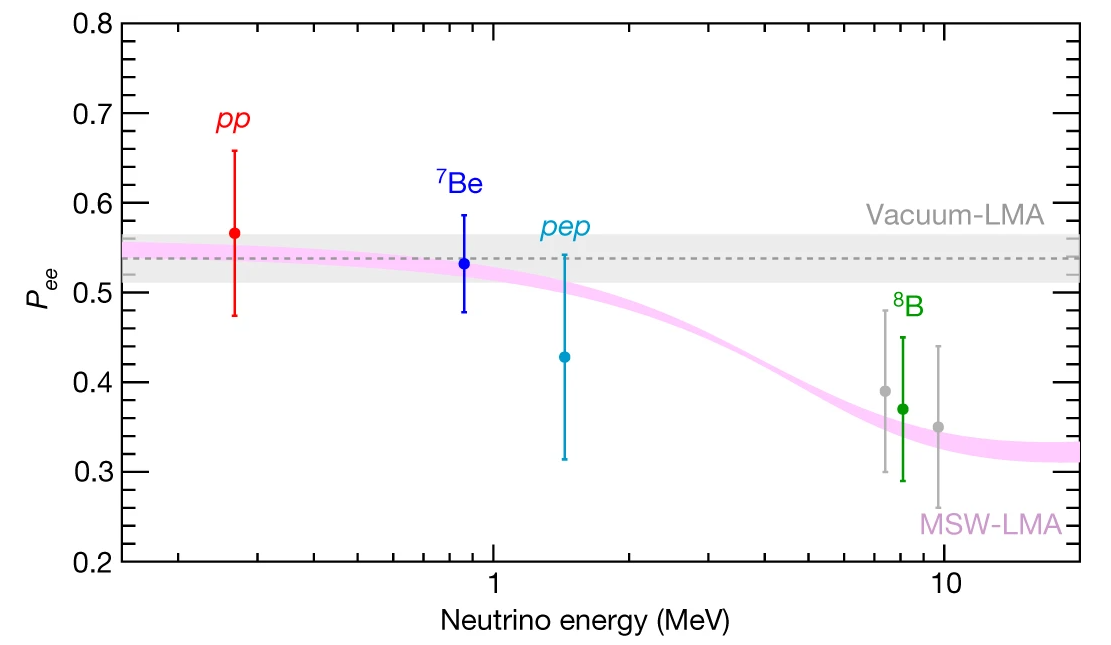
\includegraphics[width=0.8\textwidth]{1_NeutrinoTheory/Figs/borexino_pee_energy_plot.png}
    \caption[Measured survival probability versus mean neutrino energy for each solar neutrino type, as observed by Borexino]{Measured survival probability versus mean neutrino energy for each solar neutrino type, as observed by Borexino. Taken from~\cite{agostiniComprehensiveMeasurementPpchain2018}. For comparison, the expected survival probability due to vacuum oscillations and the MSW effect are shown.}
    \label{fig:pee_solar_data}
\end{figure}

Important to note is that the resonance phenomenon of the MSW effect requires a positive sign for \dmsq{} to occur, given that $0\leq\tonetwo{}\leq\pi/4$. If $\dmsq{}<0$, then in the case where $|A_{CC}|\gg |A_{res}|$, $\theta_{12}^{M}$ will be driven to 0 instead of $\pi/2$. This would lead to the survival probability of solar neutrinos increasing at higher energies, entirely counter to what is seen in data. Because of this, the sign of \dmsq{} is known to be positive, as mentioned in the previous section.

% \begin{itemize}
%     \item Describe the current phenomenological model of 3-flavour neutrino oscillations that can explain all of this evidence: the PMNS mixing matrix.
%     \item Describe also the MSW effect, which is critical for explaining solar neutrino oscillations.
%     \item Show the formula for solar neutrino oscillations, given this MSW effect in both the Sun and Earth. Note the dependence of solar neutrino oscillations on only the ``solar'' oscillation parameters. This is all particularly useful for the solar analysis chapter.
% \end{itemize}
% [3 pages]

\subsection{The Origins of Neutrino Mass}
Having seen a wide variety of experiments over many decades observe neutrino oscillations, and the phenomenology that describes them requiring at least two neutrino mass states to be non-zero, a critical question is how neutrino masses can be included into the SM. There are two different approaches to doing so. If neutrinos are given a \textit{Dirac mass term}, then a term similar to the one in Eq.~\ref{eq:SM_yukawa_leptons} is added, now using right-handed neutrino terms $\nu^{c}_{j}$:
\begin{align}
    -\mathcal{L}_{\mathrm{Dirac}} &= \sum_{i,j}y^{\nu}_{ij}\bar{L}^{i}CH\nu^{c}_{j} + \mathrm{ h.c.}\\
                              &\to \sum_{i,j}m^{\nu}_{ij}\bar{\nu}_{i,L}\nu^{c}_{j} + \mathrm{ h.c.}.
\end{align}
The $3\times3$ matrix $y^{\nu}_{ij}$ describes the Yukawa coupling strengths between the neutrinos and the charge conjugate of the Higgs doublet, $CH$. After SSB, a neutrino mass matrix is obtained $m^{\nu}_{ij} = \frac{v}{\sqrt{2}}y^{\nu}_{ij}$, which can be related to the PMNS mixing matrix~\cite{deppischChapterNeutrinosStandard2019}. %cite
The theoretical downsides of this approach are two-fold: firstly, because $v = \SI{246.22}{\GeV} \gg m_{\nu_{i}}\sim \mathcal{O}(10^{-2}\si{\eV\squared})$, this requires fine-tuning of the Yukawa coupling parameters down to values $\sim\mathcal{O}(10^{-14})$.

A second assumption needed for neutrinos to be Dirac particles is the existence of right-handed, `sterile' neutrinos. These are so-called because their right-handed nature precludes them from interacting via any of the three main fundamental forces of particle physics. The only known means by which sterile neutrinos could have any contact with the rest of the SM is via the above mass term of the Lagrangian; this implies that neutrinos could oscillate into a sterile neutrino state, for example. The LSND and MiniBooNE short-baseline neutrino experiments have seen excesses at low energies that could be explained by oscillations of a sterile neutrino with a mass splitting of $\Delta m^{2}_{41}\sim\mathcal{O}(\SI{1}{\eV\squared})$~\cite{aguilarEvidenceNeutrinoOscillations2001,aguilar-arevaloUpdatedMiniBooNENeutrino2021}; % cite LSND & MiniBooNE excess papers
however, these results seem at odds with recent results by the MicroBooNE Collaboration~\cite{abratenkoFirstConstraintsLight2023}. % cite MicroBooNE

\nomenclature{\textbf{BSM}}{Beyond the Standard Model}
An alternative approach to generating neutrino masses without needing to posit the existence of right-handed neutrino states is through a \textit{Majorana mass term}:
\begin{equation}
    \mathcal{L}_{M} = \frac{1}{2}\sum_{i,j}m^{\nu}_{ij}\nu^{T}_{i,L}C\nu_{j,L} + \mathrm{ h.c.},
\end{equation}
where there is now no longer a coupling to the Higgs field, and instead the charge conjugate of the left-handed neutrino states is used. This term breaks SM gauge symmetry, so in theories Beyond the Standard Model (BSM) that want to include such a term typically introduce a higher-order term that reduces after SSB down to the Majorana term~\cite{weinbergBaryonLeptonNonconservingProcesses1979}. % cite some relevant papers, inc. Weinberg
Many of these BSM theories, for example ones that include a so-called `Seesaw Mechanism', also have a means of explaining why neutrinos have such light masses, without having to resort to `unnatural' Yukawa coupling strengths~\cite{minkowskiEgRateOne1977}. % cite 
For this term to exist neutrinos must be a `Majorana particle', in which they are their own antiparticle, expressed mathematically as $\nu^{c} = \nu$. This is named after Ettore Majorana, who realised that a mass term such as the above could exist under these special conditions~\cite{majoranaTeoriaSimmetricaElettrone1937}. % cite Majorana

The existence of this Majorana mass term would have major consequences, beyond just allowing for neutrino masses. Crucially, the term violates lepton number, as it allows for neutrinos to annihilate one another. Fig.~\ref{fig:feynman_diagram_ovbb} shows an example of a process which violates lepton number by two, as two electrons have been created without any anti-leptons. Because all other terms in the SM conserve the `accidental' symmetry of lepton number conservation, any evidence of lepton number violation with neutrinos can provide strong evidence that neutrinos are Majorana particles.

\nomenclature{\textbf{\onbb{}}}{Neutrinoless double beta decay}
\nomenclature{\textbf{\twonbb{}}}{Two-neutrino double beta decay}
One prominent search mode for determining whether neutrinos have a Majorana mass term is by looking for \textit{neutrinoless double beta decay}, \onbb{}. This is a variant of the radioactive decay known as \textit{two-neutrino double beta decay}, \twonbb{}, and was first hypothesised by Wendell H Furry~\cite{furryTransitionProbabilitiesDouble1939}. % cite Furry paper
\twonbb{} is a nuclear process theorised by Maria Goeppert-Mayer~\cite{goeppert-mayerDoubleBetaDisintegration1935}, % cite
in which two $\beta$-decays occur simultaneously in one nucleus, generating two electrons and two electron anti-neutrinos. This is only possible in the subset of isotopes for which \twonbb{} is energetically allowed, but the usual single $\beta$-decay is not (or indeed any other form of nuclear decay).

One example of an isotope capable of \twonbb{} is \ce{^{130}Te}. Fig.~\ref{fig:bb_isobar_example} shows the mass excesses of the nuclear ground state energy levels for isotopes in the isobar $A = 130$. As can be seen, \ce{^{130}Te} is not capable of $\beta^{-}$-decay to \ce{^{130}I}, but decay via \twonbb{} down to the stable isotope \ce{^{130}Xe} is possible. This process has been observed by the CUORE experiment~\cite{adamsMeasurementEnsuremathNu2021}, % cite CUORE
and \twonbb{} has been similarly observed in a number of other isotopes such as \ce{^{76}Ge}~\cite{agostiniResultsBetaBeta2015}, % cite
\ce{^{136}Xe}~\cite{gandoPrecisionAnalysis1362019}, % cite
and \ce{^{150}Nd}~\cite{arnoldMeasurementEnsuremathNu2016}. % cite

\begin{figure}[!th]
    \centering
    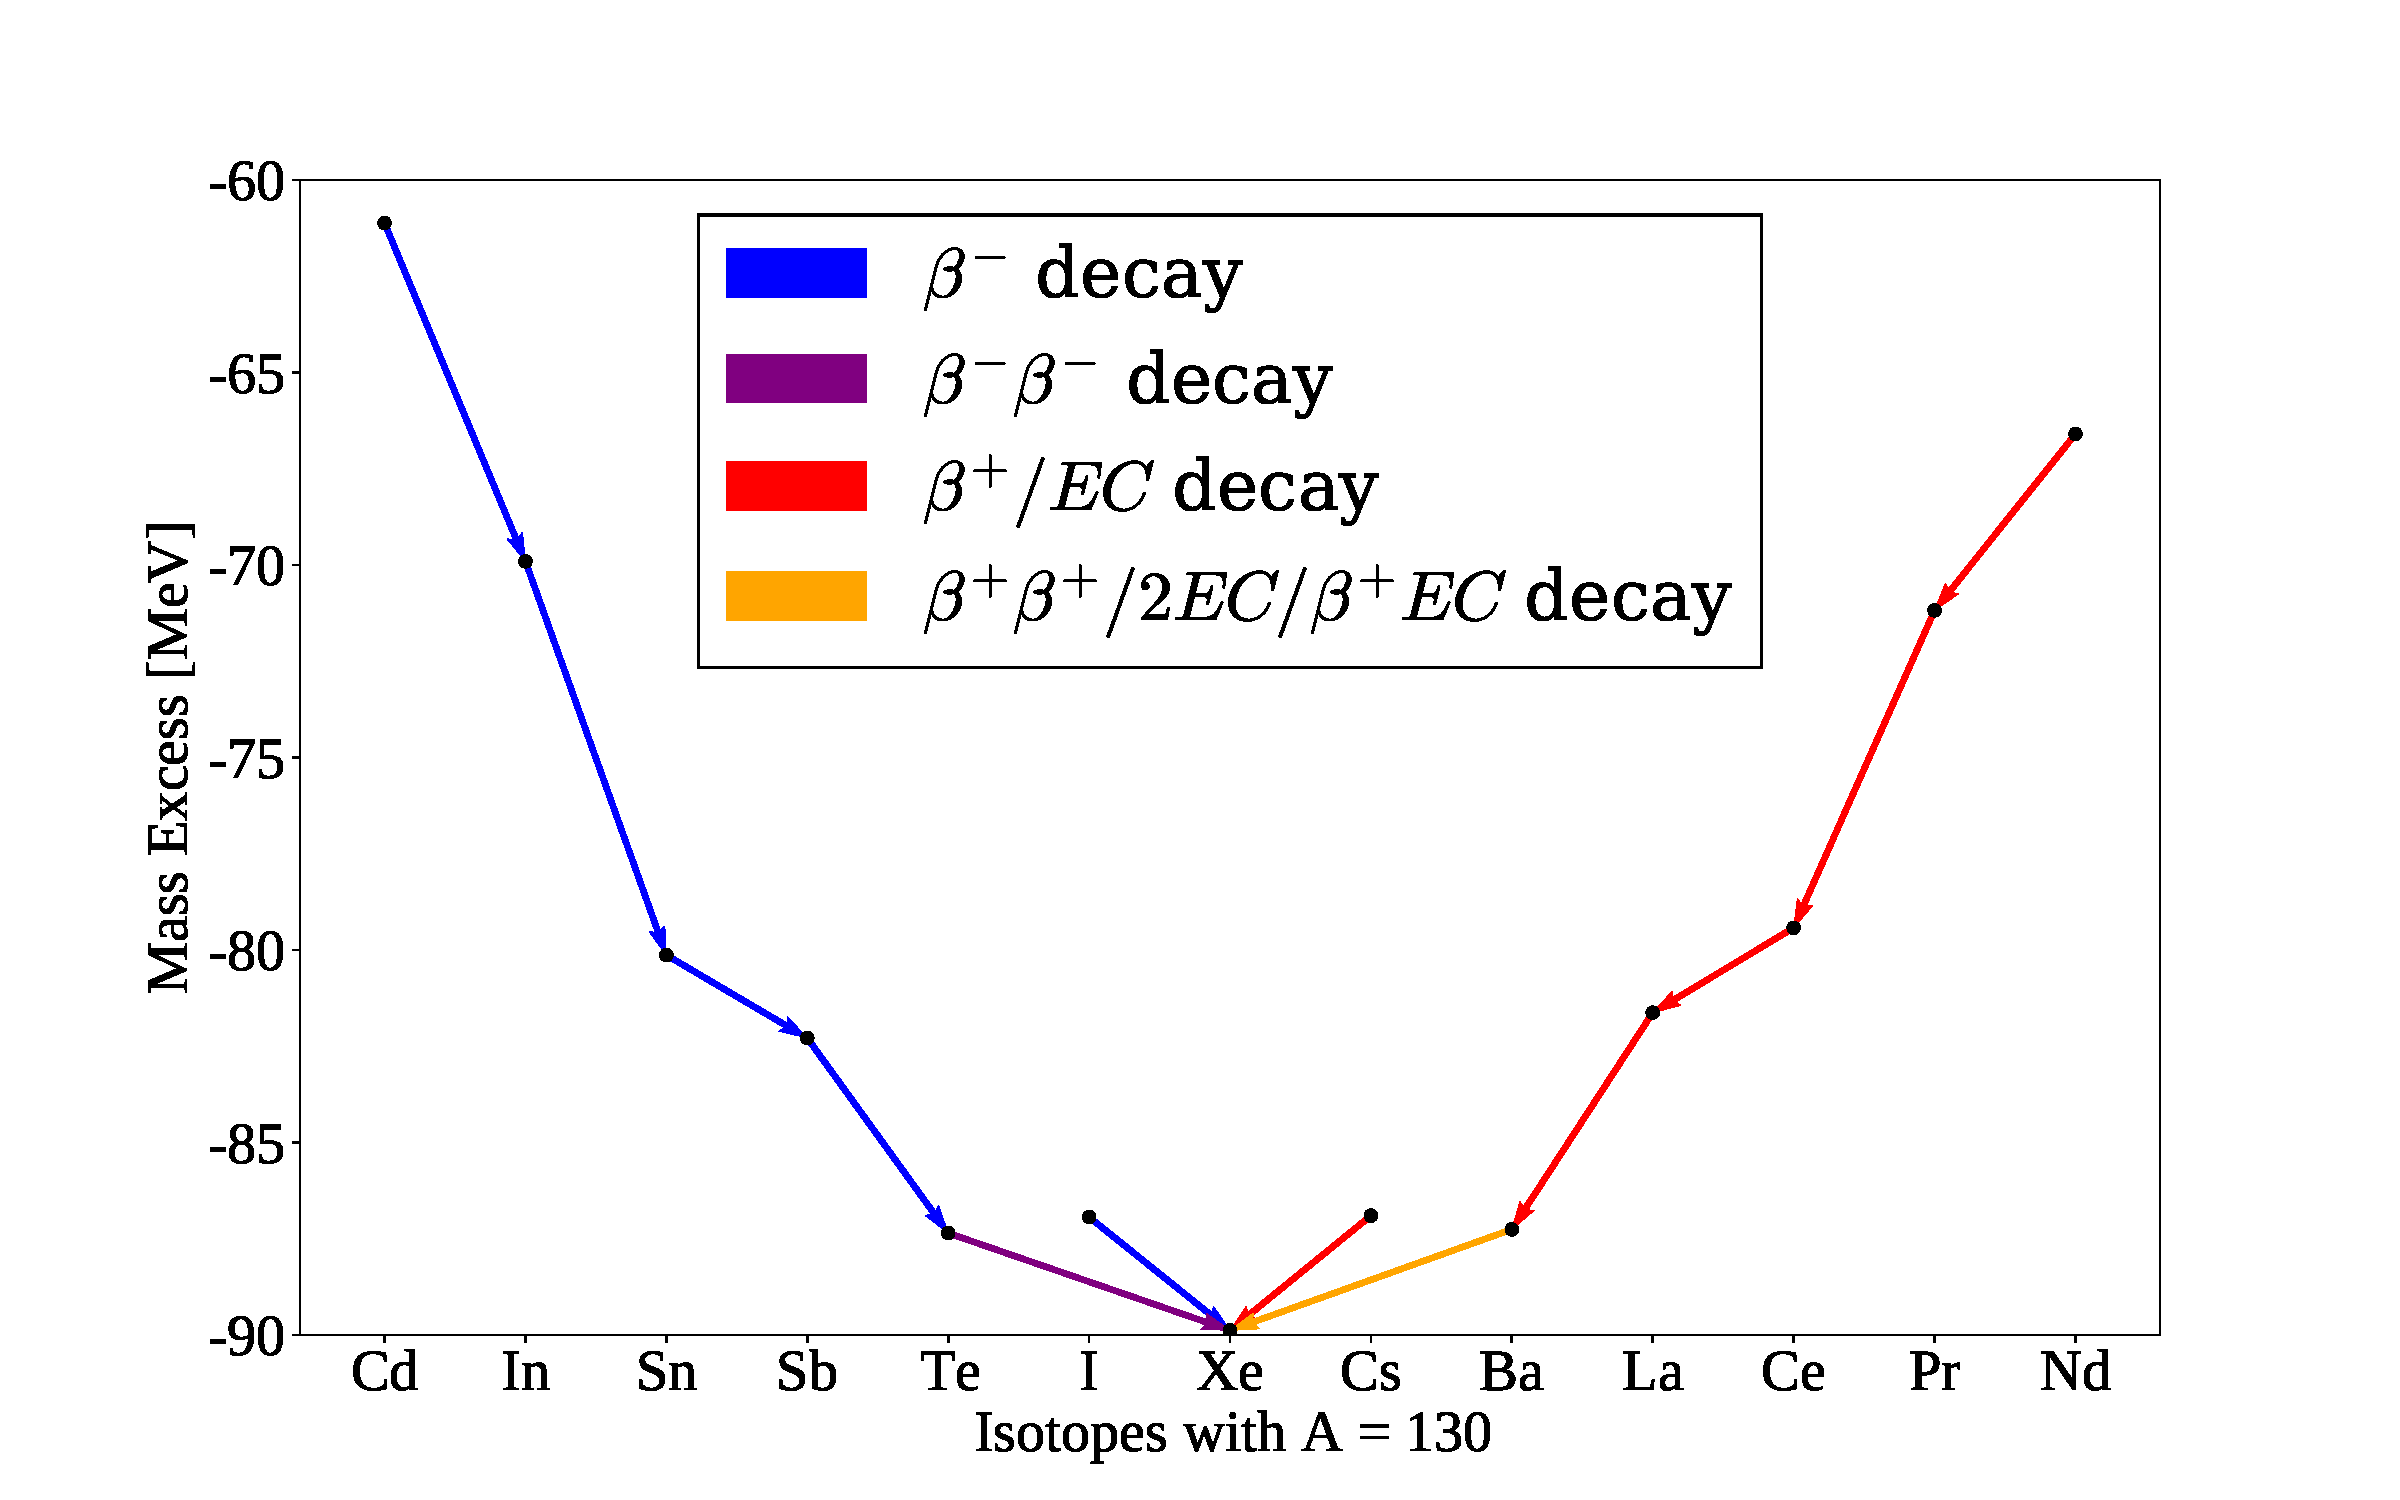
\includegraphics[width=0.8\textwidth]{1_NeutrinoTheory/Figs/A_130_isobars.pdf}
    \caption[Masses excesses of the $A = 130$ isobar, with the allowed weak decays being shown]
    {Masses excesses of the $A = 130$ isobar, from~\cite{kondevNuclearDataSheets2008}. The allowed weak decays between isotopes are shown by coloured arrows; note how both \ce{^{130}Te} and \ce{^{130}Ba} can only decay via second-order weak processes.}
    \label{fig:bb_isobar_example}
\end{figure}

Unlike \twonbb{}, \onbb{} would emit no neutrinos during the decay, and instead a virtual anti-neutrino emitted by one nucleon would be captured on another as a neutrino. Fig.~\ref{fig:feynman_diagram_ovbb} shows a Feynman diagram for this process. A theorem by J. Schechter and J.W.F. Valle~\cite{schechterNeutrinolessDoubleDecay1982} % cite
says that, as long as the weak interaction is governed by some form of local gauge theory, any observation of \onbb{} guarantees the existence of a Majorana mass term for neutrinos.

\begin{figure}[!th]
    \centering
    \begin{subfigure}{0.40\textwidth}
        \centering
        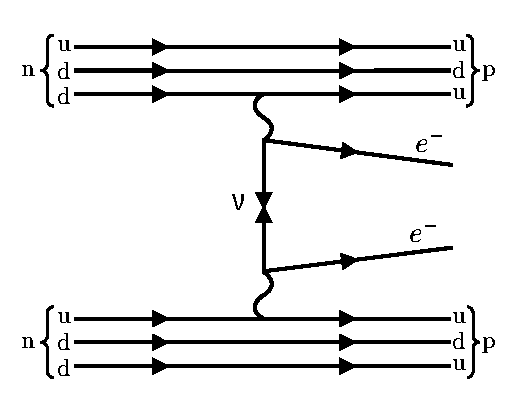
\includegraphics[width=0.95\linewidth]{1_NeutrinoTheory/Figs/feynman_diag_ovbb.pdf}
        \caption{}
        \label{fig:feynman_diagram_ovbb}
    \end{subfigure}
    \begin{subfigure}{0.59\textwidth}
        \centering
        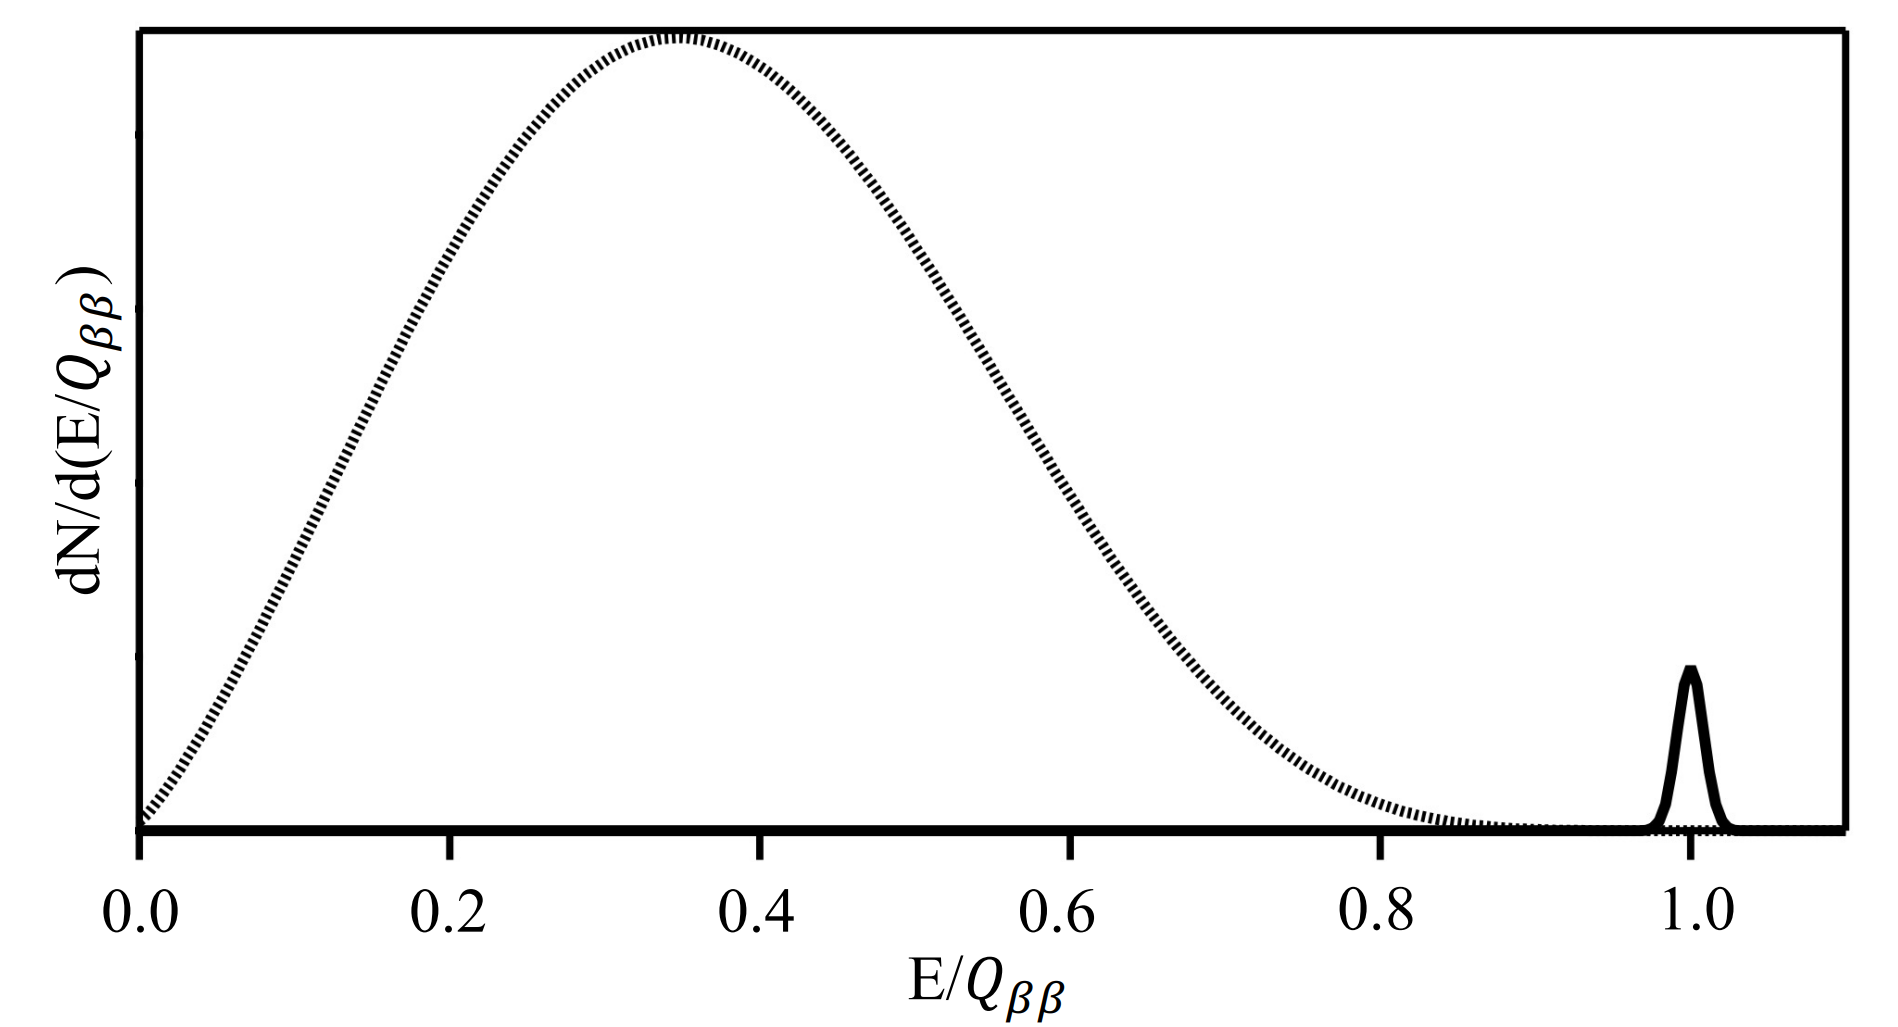
\includegraphics[width=\linewidth]{1_NeutrinoTheory/Figs/0vbb_2vbb_energy_spectrum_comparison.png}
        \caption{}
        \label{fig:energy_spectrum_bb}
    \end{subfigure}
    \caption[Feynaman diagram for \onbb{} decay, and sketch of the energy spectra for \twonbb{} and \onbb{}]
    {\textbf{(a)}: Feynman diagram for \onbb{} decay. \textbf{(b)}: Sketch of the energy spectra for \twonbb{} (dashed line) and \onbb{} decays (solid line). The $Q$-value of the decay is written here as $Q_{\beta\beta}$. Taken from~\cite{inacioDataAnalysisWater2022}.}
    \label{fig:ovbb_plots}
\end{figure}

The lack of neutrinos generated in \onbb{} compared to \twonbb{} enables a method for distinguishing between the two processes. In \twonbb{}, the energy of the decay is shared between the two electrons and two anti-neutrinos generated. Given that the anti-neutrinos rarely ever interact, the observed energy of the event will come only from the electrons (ignoring the negligble kinetic energy of the daughter nucleus). This leads to a broad observed energy spectrum. In comparison, with \onbb{} all the decay energy is passed onto the electrons, and so the observed energy spectrum will be a thin peak at the $Q$-value of the decay. This is shown schematically in Fig.~\ref{fig:energy_spectrum_bb}. As can be seen, \onbb{} can be searched for by looking for an excess of radioactive decay events generated by a \twonbb{}-decaying isotope at the $Q$-value.

No evidence of \onbb{} has been seen at the time of writing. However, numerous experiments have been searching for the decays in a variety of isotopes, and more are under construction or being planned. A summary of the current state of searches for the most prominent isotopes that could theoretically allow \onbb{} is shown in Table~\ref{tab:ovbb_current_limits}. In absence of an observation, experiments report a limit on the minimum possible half-life of \onbb{}, $T_{1/2}^{\onbb{}}$. If \onbb{} is observed, the measured half-life can be used to help determine the neutrino masses, through the formula:
\begin{equation}
    \frac{1}{T_{1/2}^{\onbb{}}} = \frac{ |m_{\beta\beta}|^{2}}{m_{e}^{2}}G_{\nu}|\mathcal{M}_{\onbb{}}|^{2},
\end{equation}
where $G_{\nu}$ and $\mathcal{M}_{\onbb{}}$ are the phase space factor and matrix elements of the decay, and $m_{\beta\beta}$ is known as the `effective \onbb{} mass', defined as:
\begin{equation}
    m_{\beta\beta} = \sum_{i=1}^{3}U_{ei}^2m_{\nu_{i}}.
\end{equation}

\begin{table}[!th]
    \centering
    \begin{tabular}{c p{3.0cm} p{4.0cm} p{0.7cm}}
        \hline
        Isotope   & $T_{1/2}^{\onbb{}}$ [years] & Experiment &   \\ \hline \hline
        \ce{^{76}Ge} & $>\num{1.8e26}$  & GERDA & \cite{agostiniFinalResultsGERDA2020} \\
        \ce{^{100}Mo} & $>\num{1.5e24}$  & CUPID-Mo & \cite{armengaudNewLimitNeutrinoless2021} \\
        \ce{^{130}Te} & $>\num{2.2e25}$  & CUORE & \cite{adamsSearchMajoranaNeutrinos2022} \\
        \ce{^{136}Xe} & $>\num{2.3e26}$  & KamLAND-Zen & \cite{abeSearchMajoranaNature2023} \\
        \hline
    \end{tabular}
    \caption[Current best limits on the half-life for \onbb{} decay for selected isotopes]
    {Current best limits on the half-life for \onbb{} decay, for a selection of isotopes. All limits given are for a 90\% CL.}
    \label{tab:ovbb_current_limits}
\end{table}

% {
% \color{blue}
% \begin{itemize}
%     \item Observed neutrino oscillations require at least two neutrino mass states to be non-zero. Given constraints of the current SM, two main ways of adding neutrino masses: a Dirac mass term (i.e. allowing for sterile neutrinos), and a Majorana mass term.
%     \item For latter, briefly describe what a Majorana particle is, and how with the Seesaw Mechanism (just the simple Type 1 described in-text) one can not only get neutrino masses but also explain their lightness relative to the other massive SM particles. Note that there exist more elaborate versions of this theory.
%     \item Furthermore, with reference to the Sakharov conditions, describe qualitatively how the Seesaw Mechanism also allows for possible leptogenesis/baryogenesis in the early Universe, and hence could explain its matter-antimatter asymmetry.
%     \item Describe briefly the nuclear physics behind double-beta decay (i.e. why it can happen at all over just normal beta decay), and then how Majorana neutrinos allow for neutrinoless double beta decay, \onbb{}.
%     \item Describe the experimental signature of \onbb{}: a spike of events of observed energy equal to the Q-value of the decay.
%     \item Note Schecter-Valle Theorem ensures that any observation of \onbb{} must be the result of neutrinos being Majorana. I.e. the Universe cannot conspire against us and have \onbb{} without Majorana neutrinos.
%     \item Very briefly note the current status of the search for \onbb{}, describing the main varieties of experimental setup seen, along with a nice canonical example of such an experiment and their best limit. In particular, the Germanium-crystal detectors such as GERDA, Xenon-TPC detectors like EXO-200, and large-scale liquid scintillators such as KamLAND-Zen.
% \end{itemize}
% [3 pages]

% [CHAPTER TOTAL: 17 pages]
% }